% =====================================================================
% PTB-XL Visual Analytics - Informe (estructura: Introducción, Trabajos relacionados, Modelos, Descripción general, Diseño visual, Resultados, Discusión, Conclusiones)
% Compilar con pdfLaTeX (Overleaf: compilador pdfLaTeX, archivo principal main.tex)
% Archivos opcionales que se leen si existen:
%   figuras/comparacion_proyecciones.png   (lo genera el notebook v3.1)
%   tabla_proyecciones.tex                 (python3 csv_a_latex.py comparacion_proyecciones.csv)
% =====================================================================
\documentclass[conference]{IEEEtran}

\usepackage[utf8]{inputenc}
\usepackage[T1]{fontenc}
\usepackage[spanish,es-noshorthands]{babel}
\usepackage{amsmath,amssymb}
\usepackage{graphicx}
\usepackage{booktabs}
\usepackage{array}
\usepackage{tabularx}
\usepackage{multirow}
\usepackage{xcolor}
\usepackage{tikz}
\usetikzlibrary{positioning}
\usepackage{url}

% colores por superclase (los mismos que usa la plataforma)
\definecolor{cNORM}{HTML}{3FA66B}
\definecolor{cMI}{HTML}{D9372B}
\definecolor{cSTTC}{HTML}{F29B38}
\definecolor{cCD}{HTML}{6FC3E3}
\definecolor{cHYP}{HTML}{3B62C9}

\newcolumntype{L}[1]{>{\raggedright\arraybackslash}p{#1}}

\begin{document}

\title{Interpretabilidad visual de la detección de infarto de miocardio en PTB-XL mediante un espacio latente aprendido}

\author{\IEEEauthorblockN{Ignacio Martín Estremadoyro Lam}
\IEEEauthorblockA{Maestría en Ciencias de la Computación\\
Universidad Nacional de San Agustín de Arequipa\\
iestremadoyro@unsa.edu.pe}
\and
\IEEEauthorblockN{Andree Eduardo Morales Pulcha}
\IEEEauthorblockA{Maestría en Ciencias de la Computación\\
Universidad Nacional de San Agustín de Arequipa\\
amoralesp@unsa.edu.pe}%
\thanks{Trabajo final del curso Ciencia de Datos y Big Data, a cargo de la Dra. Ana María Cuadros Valdivia.}}

\maketitle

\begin{abstract}
Los modelos de inteligencia artificial que leen electrocardiogramas (ECG) suelen presentarse con un número global de acierto, pero ese número no dice en qué casos se equivocan. En este trabajo construimos una plataforma de interpretabilidad visual para un modelo que detecta el infarto de miocardio en la base de datos PTB-XL: comparamos cada ECG con sus vecinos más parecidos y con su señal original para ver dónde se ubican los infartos y en qué casos el modelo falla. No usamos algoritmos de explicabilidad como SHAP o LIME. Entrenamos una red neuronal que resume cada ECG en 64 números, dibujamos esos resúmenes en un mapa de dos dimensiones y conectamos siete vistas y tres ventanas de apoyo para explorar grupos de pacientes, comprobar si los infartos se agrupan y revisar los casos en que el modelo falla. En 1.650 registros de prueba el modelo clasifica bien en general (AUC macro de 0,92--0,93), pero detecta cerca de dos de cada tres infartos (68\,\%). Con el resumen que aprende la red, el mapa recupera cerca del 57\,\% de los infartos usando solo dos coordenadas, frente a 5\,\% con la señal cruda. Al revisar los errores, vemos que el modelo detecta menos infartos anteriores (0,56 frente a 0,72 en los inferiores) y menos infartos en mujeres (0,58 frente a 0,71 en hombres). Los infartos mal clasificados tienen vecinos de otra clase (solo 13\,\% comparten la etiqueta real, frente a 76\,\% en los bien clasificados) y cambiar la distancia no los rescata, así que la causa está en lo que aprendió la red y no en la métrica. En la señal, los infartos perdidos conservan la forma general de un infarto, pero se desvían menos del latido normal típico que los detectados, sobre todo en el QRS de las derivaciones III, aVF y aVL. Son descripciones del error en este conjunto de datos, no explicaciones causales.
\end{abstract}

\begin{IEEEkeywords}
Visual Analytics, electrocardiograma, PTB-XL, espacio latente, aprendizaje contrastivo, infarto de miocardio.
\end{IEEEkeywords}

% =====================================================================
\section{Introducción}

\subsection{Contexto}
El electrocardiograma (ECG) registra la actividad eléctrica del corazón mediante sensores colocados en el cuerpo y es una de las pruebas más usadas para detectar problemas cardíacos, entre ellos el infarto de miocardio. Hoy los hospitales guardan miles de ECG en formato digital. Un ejemplo es PTB-XL \cite{wagner}, una base pública con 21.799 registros de 10 segundos, medidos con 12 sensores (llamados derivaciones) y etiquetados por cardiólogos en cinco diagnósticos generales: normal (NORM), infarto (MI), cambios en el segmento ST y la onda T (STTC), alteraciones de la conducción (CD) e hipertrofia (HYP). Varios modelos de aprendizaje profundo ya clasifican estos registros con buen desempeño \cite{strodthoff}.

Eso es útil, pero deja una pregunta práctica: si un modelo va a apoyar a un médico, ¿cómo sabemos en qué casos se equivoca? Un error del que el modelo está muy seguro es más peligroso que uno dudoso, y revisar a mano miles de señales no es viable. En lo social, un infarto que el modelo no reconoce puede retrasar la atención de un paciente; en lo computacional, estos modelos suelen reportarse con métricas globales y es poco habitual poder revisar caso por caso qué aprendieron. Hacen falta herramientas visuales que resuman a la población y que permitan bajar hasta un paciente concreto. El Cuadro~\ref{tab:glosario} resume los términos que usamos en el resto del texto.

\begin{table}[t]
\centering
\caption{Glosario de términos clave.}
\label{tab:glosario}
\small
\renewcommand{\arraystretch}{1.1}
\begin{tabular}{L{2.2cm} L{5.9cm}}
\toprule
Término & Qué significa \\
\midrule
ECG & Registro de la actividad eléctrica del corazón. \\
Derivación & Cada uno de los 12 ``ángulos'' desde los que se mide esa actividad. \\
Infarto (MI) & Daño en el músculo del corazón por falta de riego; cambia la forma de algunas ondas del ECG. \\
Embedding & Resumen numérico de un ECG (aquí, 64 números) que aprende el modelo. ECG parecidos tienen resúmenes parecidos. \\
UMAP, t-SNE & Técnicas que dibujan esos 64 números en un plano de dos dimensiones. \\
Vecinos & Los ECG cuyo resumen es más parecido al de un registro dado. \\
Recall & De todos los infartos reales, la proporción que el modelo detecta. \\
Registros de prueba & Registros que el modelo nunca vio al entrenar; sirven para evaluarlo con honestidad. \\
Caso frontera & Infarto real que el modelo no reconoce y cuyos vecinos tampoco parecen infartos. \\
\bottomrule
\end{tabular}
\end{table}

\subsection{Problema}
Nuestro punto de partida fue un experimento sencillo: entrenamos un modelo y lo probamos con registros que no había visto. El AUC macro (una medida global de acierto en la que 1 es perfecto y 0,5 equivale al azar) fue de 0,92, un buen resultado. Pero al mirar solo los infartos, el modelo reconoce cerca de dos de cada tres (68\,\%). Los demás se confunden sobre todo con ECG normales o con cambios ST-T. En los errores más claros, el modelo le da al infarto una probabilidad de entre 2 y 13\,\%, y a lo sumo 2 de sus 10 pacientes más parecidos son infartos. Esto deja tres dificultades:
\begin{enumerate}
\item \textbf{Un número global esconde dónde falla el modelo.} Hace falta ver los errores por tipo de infarto, por sexo, por edad y por paciente.
\item \textbf{Los mapas de dos dimensiones pueden engañar.} Si dibujamos los mismos datos con los que el modelo aprendió, los grupos se ven separados aunque el modelo solo los haya memorizado. Y si dibujamos la señal cruda (tiempo e intensidad) sin resumirla, puede salir una nube sin forma, porque no se captura la forma del latido.
\item \textbf{Una decisión práctica oculta información.} Para entrenar usamos solo los registros con un único diagnóstico. Eso descarta el 24\,\% de los registros diagnosticados (5.144 de 21.388) y hasta el 80\,\% de los de hipertrofia. Esa pérdida debe ser visible para quien analiza.
\end{enumerate}

La pregunta que guía el proyecto es: \emph{¿dónde se ubican los pacientes con infarto en un mapa construido por el modelo, frente a los sanos y a otras patologías, y qué casos frontera no reconoce?}

\subsection{Objetivo y aportes}
\textbf{Objetivo.} Construir una plataforma de interpretabilidad visual para un modelo que detecta infarto de miocardio en PTB-XL: ver dónde se ubican los infartos en un mapa construido a partir de lo que aprende el modelo, comparar cada caso con sus vecinos más parecidos y con su señal original, y entender en qué casos y en qué grupos de pacientes el modelo falla.

\textbf{Alcance.} Entendemos el modelo \emph{mirando ejemplos}: sus predicciones, sus probabilidades, los ECG más parecidos de cada caso (vecinos) y la señal original superpuesta. No usamos algoritmos de explicabilidad como SHAP o LIME ni medimos qué derivación o qué instante pesa más en una predicción; eso queda como trabajo futuro. Las zonas resaltadas en la ventana de comparación muestran dónde difiere la señal de un caso respecto a sus vecinos, no qué usó el modelo para decidir. La clasificación la hace la red neuronal; el método de vecinos (kNN) se usa sobre sus resúmenes de 64 números para comparar casos y revisar errores, no como clasificador de la plataforma. La revisión clínica final corresponde a una persona especialista.

Los aportes son:
\begin{enumerate}
\item Una evaluación honesta: separamos entrenamiento, validación y prueba según el protocolo oficial y comparamos tres sistemas (una red neuronal, la misma red con una pérdida contrastiva y un modelo clásico más simple). El modelo detecta cerca de dos de cada tres infartos (68\,\%).
\item Un mapa de dos dimensiones con los 10 ECG más parecidos de cada registro y un índice de cuántos comparten el diagnóstico. Con el resumen que aprende la red, el mapa recupera cerca del 57\,\% de los infartos, frente a 5\,\% con la señal cruda y 19\,\% con características hechas a mano.
\item Una interfaz de tres niveles (general, intermedio y detalle) para explorar grupos de pacientes, comprobar si los infartos se agrupan y revisar los casos frontera, con vistas enlazadas: al elegir errores en la matriz de confusión se resaltan en el mapa y se abre su señal junto a la de sus vecinos.
\item Un análisis de los errores en infartos por tipo de infarto, sexo, edad, ruido y etapa, donde se ve que se detectan peor los infartos anteriores, los de mujeres y los de etapa desconocida.
\item Un estudio de por qué fallan los infartos mal clasificados: comparamos cuatro distancias, medimos qué tan lejos están sus vecinos y los contrastamos con dos algoritmos de agrupamiento (K-means y DBSCAN).
\item Una comparación en la señal: una ventana que pone el latido medio de un caso frente a sus 10 vecinos, un mapa agregado que muestra que los infartos perdidos conservan la forma de un infarto, pero con una huella más débil frente al ECG normal, sobre todo en el QRS de las derivaciones III, aVF y aVL, y una ventana de pruebas de apoyo que reúne en la propia plataforma los resultados sobre distancias, vecinos lejanos, agrupamientos y preprocesamiento.
\end{enumerate}

% =====================================================================
\section{Trabajos relacionados}
Revisamos qué se ha hecho en dos frentes: los modelos que leen ECG y los sistemas de análisis visual. Al final, el Cuadro~\ref{tab:comparativo} los compara con nuestra propuesta.

\subsection{Modelos para ECG y resúmenes numéricos de las señales}
PTB-XL \cite{wagner} es la base pública de ECG de 12 derivaciones más usada para clasificar diagnósticos. Strodthoff et~al. \cite{strodthoff} compararon muchas redes neuronales sobre esta base y obtuvieron un AUC macro superior a 0,92 en los cinco diagnósticos generales. Hannun et~al. \cite{hannun} mostraron que una red profunda puede detectar arritmias con un nivel parecido al de cardiólogos usando ECG de un solo sensor. Ambos trabajos presentan sus resultados como tablas de números, sin una herramienta para revisar los errores caso por caso.

Para que un modelo organice mejor lo que aprende existe el aprendizaje contrastivo supervisado \cite{khosla}: durante el entrenamiento se le pide que ponga cerca a los ejemplos de la misma clase y lejos a los de clases distintas. En ECG, CLOCS \cite{kiyasseh} usa una idea parecida entre derivaciones, momentos y pacientes. En visualización, Luo et~al. \cite{luo} combinan aprendizaje contrastivo con otras redes para resumir series de calidad del aire y dibujarlas con t-SNE. Para pasar de muchos números a un plano se usan UMAP \cite{mcinnes} y t-SNE \cite{vandermaaten}. Ambas conservan bien los vecindarios, pero las distancias exactas en el plano no son fiables; por eso comprobamos lo que vemos con los vecinos calculados en el espacio original.

\subsection{Análisis visual de series temporales y de modelos}
AirLens \cite{qu} ayuda a explorar cómo evoluciona la calidad del aire en un conjunto de ciudades y la organiza en tres módulos (selección de datos, inspección de patrones y análisis de la evolución). Luo et~al. \cite{luo} conectan un mapa t-SNE, donde se pueden seleccionar puntos con un lazo, con gráficos de series y de atributos. Voila \cite{cao} combina análisis de tensores y detección de anomalías para datos que llegan continuamente. CrimAnalyzer \cite{alvarenga} enlaza un mapa, vistas temporales y vistas radiales para estudiar delitos, y define de forma explícita qué tarea resuelve cada vista. AQX \cite{velumani} se dedica a explicar un pronóstico de calidad del aire mostrando cuánto aporta cada variable de entrada. Nuestro trabajo toma otro camino: no abre el modelo, sino que revisa sus resultados y sus errores.

\subsection{Cuadro comparativo}
\begin{table*}[t]
\centering
\caption{Comparación de los trabajos revisados con nuestra propuesta.}
\label{tab:comparativo}
\scriptsize
\renewcommand{\arraystretch}{1.15}
\begin{tabular}{L{2.4cm} L{3.2cm} L{3.6cm} L{3.3cm} L{4.5cm}}
\toprule
Trabajo & Dominio y datos & Modelo o extracción de características & Visualización principal & Limitación frente a nuestro problema \\
\midrule
Strodthoff et~al. (2021) \cite{strodthoff} & ECG de 12 derivaciones, PTB-XL & CNN y otras arquitecturas (benchmark) & Tablas de métricas & Sin exploración visual ni análisis de errores por caso \\
Hannun et~al. (2019) \cite{hannun} & ECG ambulatorio de una derivación & CNN de 34 capas & Métricas por clase de ritmo & Sin interfaz; no audita fallos individuales \\
Luo et~al. (2024) \cite{luo} & Calidad del aire, series multivariadas & Aprendizaje contrastivo y transformer, con t-SNE & Dispersión 2D con lazo y vistas enlazadas & Dominio ambiental; no hay un clasificador que revisar \\
AirLens (2022) \cite{qu} & Calidad del aire en aglomeraciones urbanas & Agrupamiento de patrones & Vistas multinivel & Se centra en patrones espacio-temporales, no en errores de un modelo \\
Voila (2017) \cite{cao} & Datos espacio-temporales en flujo & Análisis tensorial y detección de anomalías & Vistas enlazadas de anomalías & Detecta anomalías de los datos, no de un clasificador \\
CrimAnalyzer (2020) \cite{alvarenga} & Delitos en São Paulo & Detección de \emph{hotspots} & Mapa, vistas temporales y radiales & Sin modelo predictivo que revisar \\
AQX (2022) \cite{velumani} & Pronóstico de calidad del aire & ConvLSTM y contribución de variables & Vistas de contribución de variables & Explica un pronóstico (regresión) por importancia de variables; no audita errores de un clasificador; dominio no clínico \\
\midrule
\textbf{Nuestra propuesta} & ECG de 12 derivaciones, PTB-XL (16.244 registros) & CNN 1D con pérdida contrastiva, comparada con un baseline clásico & Mapa latente, matriz de confusión, ECG y vecinos & Una superclase por registro; sin validación clínica \\
\bottomrule
\end{tabular}
\end{table*}

\textbf{Qué falta en la literatura revisada.} Los sistemas de análisis visual que encontramos se aplican a datos ambientales o urbanos y se centran en descubrir patrones o en explicar pronósticos por dentro. Los trabajos sobre ECG se centran en el rendimiento global. Nuestra propuesta lleva el análisis visual a la interpretación de un clasificador clínico: dónde caen los infartos en el espacio aprendido, quiénes son sus vecinos y a qué distancia, y por qué el modelo no reconoce ciertos casos.

% =====================================================================
\section{Modelos}
En esta sección describimos las piezas del modelo: la red que lee el ECG, la forma de entrenarla, el modelo clásico con el que la comparamos y el paso del resumen numérico al mapa. Lo hacemos sin entrar en demasiado detalle matemático. El Cuadro~\ref{tab:config} reúne los ajustes principales.

\subsection{La red que lee el ECG}
La entrada es la señal completa: 12 derivaciones con 1.000 instantes cada una (10 segundos a 100 mediciones por segundo). Una red neuronal convolucional 1D recorre la señal con pequeños ``filtros'' que aprenden a reconocer formas del latido, como el pico QRS o el tramo ST. Usamos cuatro bloques de estos filtros. Al final, un paso de atención combina la información de los distintos instantes en un solo resumen. Lo usamos solo para eso: no lo interpretamos como una explicación de la decisión del modelo.

La red entrega dos cosas: un resumen de 64 números (el \emph{embedding}) y una probabilidad para cada una de las cinco clases.

\subsection{Cómo aprende: dos lecciones a la vez}
El modelo aprende con dos lecciones a la vez. La primera es la habitual, la \emph{entropía cruzada}: acertar la clase de cada ECG. La segunda es la \emph{pérdida contrastiva supervisada} \cite{khosla}: acercar los resúmenes de ECG con el mismo diagnóstico y alejar los de diagnósticos distintos, como imanes que atraen a los iguales y repelen a los distintos. Un ajuste (la ``temperatura'') controla qué tan estricta es esa separación. Las dos lecciones se mezclan a partes iguales: la pérdida total es el promedio de ambas.

Para dar variedad, cada ECG se muestra dos veces con pequeñas alteraciones (cambio de amplitud, algo de ruido y un ligero desplazamiento en el tiempo). Como hay muchos más ECG normales que de otras clases, al armar cada lote de entrenamiento damos más oportunidades a las clases pequeñas. Entrenamos hasta que el resultado en los datos de validación deja de mejorar.

\begin{table}[t]
\centering
\caption{Ajustes principales del entrenamiento.}
\label{tab:config}
\small
\renewcommand{\arraystretch}{1.1}
\begin{tabular}{L{2.6cm} L{5.5cm}}
\toprule
Elemento & Valor \\
\midrule
Entrada & 12 derivaciones $\times$ 1.000 instantes \\
Red & 4 bloques (32, 64, 128 y 128 filtros) \\
Resumen (embedding) & 64 números \\
Pérdida & entropía cruzada + contrastiva (mitad y mitad; temperatura 0,1) \\
Variaciones & amplitud $\pm10\,\%$, ruido, desplazamiento de hasta 0,5~s \\
Balanceo & muestreo proporcional a $n_c^{-1/2}$ \\
Optimizador & AdamW, tasa $10^{-3}$, lotes de 128 \\
Parada & hasta 60 épocas; se detiene si el AUC macro de validación no mejora en 12 épocas \\
\bottomrule
\end{tabular}
\end{table}

\subsection{Un modelo más simple como punto de comparación}
Para saber si la red neuronal realmente aporta, la comparamos con un método clásico. Calculamos 124 características a mano: diez estadísticos por derivación (por ejemplo, promedio, máximo, mínimo y cuánta energía hay en tres bandas de frecuencia) y cuatro medidas del ritmo del corazón. Un clasificador de tipo \emph{gradient boosting} (muchos árboles de decisión pequeños) aprende a clasificar a partir de ellas.

\subsection{Del resumen al mapa: proyección y vecinos}
Para dibujar los resúmenes de 64 números en un plano usamos UMAP \cite{mcinnes}, ajustado solo con los registros de entrenamiento y aplicado después a validación y prueba, y t-SNE \cite{vandermaaten}, que no puede ubicar puntos nuevos y por eso se calcula con todos los registros. Para cada ECG buscamos además sus 10 vecinos más parecidos entre los registros de entrenamiento, y calculamos qué fracción de ellos comparte su diagnóstico:
\begin{equation}
\kappa_i=\frac{1}{10}\sum_{j\in N_{10}(i)}\mathbf{1}[y_j=y_i].
\label{eq:acuerdo}
\end{equation}
Un infarto con $\kappa_i$ bajo cuya predicción no es infarto es lo que llamamos un caso frontera.

Para saber si un mapa es bueno, medimos sobre los registros de prueba: cuánto acierta un clasificador sencillo (kNN) usando solo las dos coordenadas; el \emph{silhouette}, que indica qué tan separados quedan los grupos; qué proporción de infartos se recupera y su AUC; y la \emph{trustworthiness}, que revisa si los puntos cercanos en el mapa también lo eran en el espacio original.

\subsection{En qué se diferencia de otros modelos}
Los modelos de referencia en PTB-XL \cite{strodthoff} se comparan por sus métricas globales. Aquí el modelo es solo la base de la revisión: importa menos su acierto que el espacio de 64 números que produce, que se puede dibujar, consultar por vecinos y revisar caso por caso. Además, combinamos la entropía cruzada con la idea contrastiva usada en CLOCS \cite{kiyasseh} y en Luo et~al. \cite{luo}, y medimos su aporte frente a la misma red sin ella (sección~VII-B). No usamos un método de explicabilidad como SHAP o LIME.

% =====================================================================
\section{Descripción general del sistema}

\subsection{Los datos}
Usamos PTB-XL \cite{wagner}, con 21.799 registros de ECG de 12 derivaciones y 10 segundos, en su versión a 100 mediciones por segundo. De ellos, 411 no tienen diagnóstico general y 21.388 sí; de estos, 16.244 tienen un solo diagnóstico y 5.144 tienen varios a la vez. El Cuadro~\ref{tab:clases} muestra cuánto se pierde al quedarnos con un solo diagnóstico por registro, y el Cuadro~\ref{tab:cooc} qué diagnósticos suelen aparecer juntos.

\begin{table}[t]
\centering
\caption{Cuántos registros hay de cada diagnóstico y cuántos se pierden al quedarnos solo con los que tienen un único diagnóstico.}
\label{tab:clases}
\small
\begin{tabular}{lrrr}
\toprule
Clase & Registros & Un solo diagnóstico & Descartado (\%) \\
\midrule
NORM & 9.514 & 9.069 & 4,7 \\
MI   & 5.469 & 2.532 & 53,7 \\
STTC & 5.235 & 2.400 & 54,2 \\
CD   & 4.898 & 1.708 & 65,1 \\
HYP  & 2.649 & 535   & 79,8 \\
\bottomrule
\end{tabular}
\end{table}

\begin{table}[t]
\centering
\caption{Cuántos registros comparten dos diagnósticos a la vez (21.388 registros con diagnóstico). La diagonal es el total de cada clase.}
\label{tab:cooc}
\small
\begin{tabular}{lrrrrr}
\toprule
 & NORM & MI & STTC & CD & HYP \\
\midrule
NORM & 9.514 & 1 & 33 & 415 & 5 \\
MI   & 1 & 5.469 & 1.339 & 1.794 & 818 \\
STTC & 33 & 1.339 & 5.235 & 1.066 & 1.509 \\
CD   & 415 & 1.794 & 1.066 & 4.898 & 787 \\
HYP  & 5 & 818 & 1.509 & 787 & 2.649 \\
\bottomrule
\end{tabular}
\end{table}

\subsection{Preparación de la señal}
Antes de entrenar limpiamos la señal con un filtro que quita el vaivén lento de la línea base (por ejemplo, el que causa la respiración) y el ruido rápido, conservando las frecuencias entre 0,5 y 40~Hz y sin desplazar la señal en el tiempo. Luego normalizamos cada derivación con el promedio y la desviación de los datos de entrenamiento, de modo que las amplitudes sigan siendo comparables entre pacientes.

Dividimos los datos con el protocolo oficial de PTB-XL: los grupos 1 a 8 para entrenar (12.957 registros), el 9 para validar (1.637) y el 10 para probar (1.650: NORM 912, MI 256, STTC 242, CD 184 e HYP 56). Este protocolo coloca todos los registros de un mismo paciente en el mismo grupo, lo que evita que el modelo vea al mismo paciente al entrenar y al evaluar.

\subsection{Datos faltantes y ruido}
Antes de entrenar revisamos qué datos faltaban o venían con problemas y decidimos qué hacer con cada caso (Cuadro~\ref{tab:calidad}). La regla general fue no inventar valores: preferimos quitar un registro o marcarlo antes que rellenarlo.

\begin{table}[t]
\centering
\caption{Problemas de calidad de datos y qué hicimos con cada uno.}
\label{tab:calidad}
\small
\renewcommand{\arraystretch}{1.1}
\begin{tabular}{L{2.5cm} L{5.6cm}}
\toprule
Problema & Decisión \\
\midrule
411 registros sin diagnóstico general & Se descartan: sin etiqueta no sirven para entrenar ni para evaluar. \\
5.144 registros con varios diagnósticos & Se descartan, para que cada punto del mapa tenga una sola clase (ver Cuadro~\ref{tab:clases}). \\
Etapa del infarto desconocida (288 de 489 infartos en validación y prueba) & Se conserva como un grupo propio llamado ``desconocida'', sin imputar. \\
Valores ausentes en la señal & Se sustituyen por cero antes de filtrar. \\
Ruido anotado (deriva de la línea base, ruido estático, ráfagas o problemas de electrodos) & Se conserva el registro y se marca como ``con ruido''; el filtro atenúa la deriva y el ruido rápido. \\
Edades mayores de 89 años & PTB-XL las guarda con un valor artificial para proteger la privacidad; las agrupamos en ``90 o más''. \\
\bottomrule
\end{tabular}
\end{table}

Eliminamos solo cuando faltaba la etiqueta o el registro era ambiguo. Para la etapa del infarto no imputamos, porque no sabemos por qué falta; podría depender de otras variables del paciente (MAR) o de algo que no se registró (MNAR), y rellenarla con la etapa más frecuente podría crear una conclusión falsa. De hecho, los infartos de etapa desconocida se detectan peor (Cuadro~\ref{tab:errores}), así que mantenerlos visibles es parte del análisis. Tampoco eliminamos valores atípicos de la señal: un latido extraño puede ser justamente lo que se quiere revisar.

\subsection{Tareas de análisis}
Los usuarios que imaginamos son cardiólogos investigadores y científicos de datos clínicos que revisan un clasificador de ECG. Trabajan con registros etiquetados, datos del paciente (edad, sexo, tipo y etapa del infarto, presencia de ruido) y lo que el modelo predice. Necesitan decidir si pueden confiar en el modelo para detectar infartos y en qué grupos de pacientes falla. De esa necesidad salen tres preguntas, que convertimos en tres tareas:
\begin{itemize}
\item \textbf{T1. Explorar cohortes.} Explorar y filtrar los registros por diagnóstico, conjunto de datos (entrenamiento, validación o prueba), sexo y edad, para comparar cuántos hay de cada clase y qué diagnósticos aparecen juntos.
\item \textbf{T2. Comprobar si los infartos se agrupan.} Evaluar si los infartos forman una región propia en el mapa frente a los sanos y a las demás patologías, comparando el diagnóstico real con la predicción en los registros de prueba.
\item \textbf{T3. Revisar los casos frontera.} Inspeccionar los infartos mal clasificados o rodeados de vecinos de otra clase, comparando su ECG con el de sus vecinos más parecidos y con las características de su grupo (tipo de infarto, sexo, edad y ruido).
\end{itemize}

\subsection{Pipeline de la propuesta}
La Fig.~\ref{fig:pipeline} muestra el recorrido de los datos: partimos de PTB-XL, nos quedamos con los registros de un solo diagnóstico y los dividimos en entrenamiento, validación y prueba; limpiamos la señal; entrenamos el modelo; proyectamos sus resúmenes a un mapa y calculamos los vecinos; analizamos los errores; y por último mostramos todo en la plataforma. El cálculo pesado se hace de antemano en un notebook. El servidor (FastAPI) solo entrega los resultados ya calculados y la página web (D3.js) los dibuja y conecta entre sí; el mapa se dibuja en un \emph{canvas} para que se mueva con fluidez con miles de puntos.

\begin{figure*}[t]
\centering
\resizebox{\textwidth}{!}{%
\begin{tikzpicture}[
  caja/.style={draw=black!60, rounded corners=2pt, align=center, minimum height=1.9cm, text width=2.4cm, font=\scriptsize, fill=blue!6},
  flecha/.style={-stealth, thick, black!70}]
\node[caja] (a) {\textbf{1. Ingesta}\\PTB-XL\\21.799 registros\\100~Hz, 12 deriv.};
\node[caja, right=0.3cm of a] (b) {\textbf{2. Datos de trabajo}\\16.244 con un solo diagnóstico\\grupos 1--8 / 9 / 10};
\node[caja, right=0.3cm of b] (c) {\textbf{3. Limpieza de la señal}\\filtro 0,5--40~Hz\\y normalización};
\node[caja, right=0.3cm of c, fill=orange!10] (d) {\textbf{4. Modelo}\\red neuronal 1D\\con pérdida contrastiva};
\node[caja, right=0.3cm of d, fill=orange!10] (e) {\textbf{5. Mapa}\\resumen de 64 números\\UMAP y t-SNE en 2D\\vecinos e índice $\kappa$};
\node[caja, right=0.3cm of e] (f) {\textbf{6. Errores}\\infartos no detectados\\por tipo, sexo, edad,\\ruido y etapa};
\node[caja, right=0.3cm of f, fill=green!8] (g) {\textbf{7. Plataforma}\\FastAPI y D3.js\\7 vistas conectadas};
\foreach \x/\y in {a/b,b/c,c/d,d/e,e/f,f/g} \draw[flecha] (\x) -- (\y);
\end{tikzpicture}}
\caption{Pipeline de la propuesta. Las etapas 1 a 6 se ejecutan sin conexión en un notebook; la etapa 7 sirve los resultados.}
\label{fig:pipeline}
\end{figure*}

% =====================================================================
\section{Diseño visual}

\subsection{Visión global}
La plataforma cabe en una sola pantalla y tiene siete vistas conectadas, organizadas en tres niveles (Fig.~\ref{fig:interfaz}); en la plataforma los niveles se rotulan macro, meso y micro. A la izquierda está el nivel general (vistas A y B), arriba a la derecha el nivel intermedio (vistas C, D y E) y abajo a la derecha el nivel de detalle (vistas F y G). Tres ventanas emergentes completan el análisis de un caso y del conjunto: una compara el caso con sus 10 vecinos (H), otra resume dónde difieren los infartos perdidos de los detectados (I) y la tercera reúne las pruebas de apoyo con las que se descartaron otras explicaciones (J). La persona que analiza empieza por los grupos de pacientes (T1), comprueba en el mapa y en la matriz de confusión si los infartos se agrupan (T2) y termina en un paciente concreto, comparándolo con sus vecinos (T3). Todas las vistas usan los mismos colores para cada diagnóstico y se actualizan juntas cuando se filtra o se selecciona algo.

\begin{figure*}[t]
\centering
\newcommand{\vista}[6]{%
  \draw[rounded corners=2pt, fill=white, draw=black!50] (#1,#2) rectangle (#3,#4);
  \node[anchor=north west, font=\scriptsize\bfseries, inner sep=2pt] at (#1,#4) {#5};
  \node[anchor=south east, font=\tiny, text=blue!60!black, inner sep=2pt] at (#3,#2) {#6};}
\resizebox{0.95\textwidth}{!}{%
\begin{tikzpicture}[x=1cm,y=1cm]
% --- A: composición de cohortes
\vista{0}{5.0}{3.8}{9.6}{A. Cohortes}{GENERAL · T1}
\node[anchor=north west, font=\tiny, text width=3.5cm] at (0.1,8.9) {Todos \; Train \; Val \; \fbox{Test}\\Sexo $\blacktriangledown$ \; Edad \; \fbox{MI mal clasif.}};
\begin{scope}[shift={(1.9,7.0)}]
  \fill[cNORM] (0,0) -- (0:1) arc (0:200:1) -- cycle;
  \fill[cMI]   (0,0) -- (200:1) arc (200:256:1) -- cycle;
  \fill[cSTTC] (0,0) -- (256:1) arc (256:309:1) -- cycle;
  \fill[cCD]   (0,0) -- (309:1) arc (309:347:1) -- cycle;
  \fill[cHYP]  (0,0) -- (347:1) arc (347:360:1) -- cycle;
  \fill[white] (0,0) circle (0.55);
\end{scope}
\node[anchor=north west, font=\tiny, text width=3.5cm] at (0.1,5.95) {Exactitud de la selección y recall de MI};
% --- B: coocurrencia
\vista{0}{0}{3.8}{4.8}{B. Matriz de coocurrencia}{GENERAL · T1}
\foreach \i in {0,...,4}{\foreach \j in {0,...,4}{%
  \ifnum\i=\j \fill[black!25] (0.7+0.5*\j,3.7-0.5*\i) rectangle ++(0.45,0.45);
  \else \fill[orange!45] (0.7+0.5*\j,3.7-0.5*\i) rectangle ++(0.45,0.45);\fi}}
\node[anchor=north west, font=\tiny, text width=3.5cm] at (0.1,1.15) {Filas y columnas: NORM, MI, STTC, CD, HYP};
% --- C: mapa latente
\vista{4.0}{3.9}{11.4}{9.6}{C. Mapa del espacio latente}{INTERMEDIO · T2 · T3}
\node[anchor=north west, font=\tiny] at (4.1,8.9) {UMAP $\blacktriangledown$ \quad Color: real $\blacktriangledown$ \quad Lazo \quad Zoom};
\fill[cNORM, opacity=.55] (8.9,7.2) ellipse (1.9 and 1.1);
\fill[cMI,   opacity=.6]  (5.6,5.6) ellipse (1.2 and 0.9);
\fill[cSTTC, opacity=.6]  (8.0,4.7) ellipse (1.0 and 0.6);
\fill[cCD,   opacity=.6]  (5.5,7.9) ellipse (0.8 and 0.5);
\fill[cHYP,  opacity=.6]  (7.0,6.3) ellipse (0.5 and 0.3);
\draw[black, thick] (7.7,4.6) circle (0.17);
\draw[black!70] (7.7,4.6) -- (5.8,5.5) (7.7,4.6) -- (8.1,4.9) (7.7,4.6) -- (7.5,4.8);
\draw[dashed, blue!60!black] (4.6,6.7) .. controls (5.4,7.1) and (6.3,6.5) .. (6.6,5.6) .. controls (6.4,4.8) and (5.0,4.7) .. (4.6,5.4) -- cycle;
\node[font=\tiny, anchor=west] at (7.9,4.45) {caso frontera y vecinos};
% --- D: matriz de confusión
\vista{11.6}{6.7}{17.4}{9.6}{D. Matriz de confusión}{INTERMEDIO · T2 · T3}
\foreach \i in {0,...,4}{\foreach \j in {0,...,4}{%
  \ifnum\i=\j \fill[blue!55] (12.0+0.45*\j,8.55-0.42*\i) rectangle ++(0.4,0.37);
  \else \fill[blue!12] (12.0+0.45*\j,8.55-0.42*\i) rectangle ++(0.4,0.37);\fi}}
\fill[cSTTC] (12.0+0.45*2,8.55-0.42*1) rectangle ++(0.4,0.37);
\node[anchor=north west, font=\tiny, text width=3.1cm] at (14.5,8.9) {Filas: real\\Columnas: predicha\\Clic en una celda: se resalta en el mapa};
% --- E: errores de MI por subgrupo
\vista{11.6}{3.9}{17.4}{6.5}{E. Errores de MI por subgrupo}{INTERMEDIO · T3}
\foreach \k/\w/\t in {0/2.6/Anterior,1/3.3/Inferior,2/1.1/Lateral}{%
  \node[anchor=east, font=\tiny] at (13.5,5.65-0.5*\k) {\t};
  \fill[cMI, opacity=.75] (13.6,5.55-0.5*\k) rectangle ++(\w,0.25);}
\draw[dashed] (16.1,4.2) -- (16.1,5.9);
% --- F: ficha del paciente
\vista{4.0}{0}{8.6}{3.7}{F. Ficha y vecinos}{DETALLE · T3}
\node[anchor=north west, font=\tiny, text width=4.2cm] at (4.1,3.0) {ECG (id): sexo, edad, subtipo\\\textcolor{cMI}{Real: MI} \; \textcolor{cSTTC}{Modelo: STTC}};
\foreach \k/\w/\c in {0/0.5/cNORM,1/0.3/cMI,2/2.4/cSTTC}{%
  \fill[\c] (4.2,1.85-0.3*\k) rectangle ++(\w,0.17);}
\node[anchor=north west, font=\tiny, text width=4.2cm] at (4.1,1.0) {Vecinos con la misma etiqueta: 0 de 10};
% --- G: señal ECG
\vista{8.8}{0}{17.4}{3.7}{G. Señal ECG}{DETALLE · T3}
\node[anchor=north west, font=\tiny] at (8.9,3.0) {Derivación II $\blacktriangledown$ \quad Comparar con un vecino $\blacktriangledown$};
\draw[black!80, thick] (9.0,1.6) -- (9.6,1.6) -- (9.7,2.3) -- (9.8,0.9) -- (9.9,1.6) -- (10.7,1.6) -- (10.8,1.8) -- (11.0,1.6) -- (11.9,1.6) -- (12.0,2.3) -- (12.1,0.9) -- (12.2,1.6) -- (13.0,1.6) -- (13.1,1.8) -- (13.3,1.6) -- (14.2,1.6) -- (14.3,2.3) -- (14.4,0.9) -- (14.5,1.6) -- (15.3,1.6) -- (15.4,1.8) -- (15.6,1.6) -- (17.2,1.6);
\draw[black!35, thick] (9.0,1.5) -- (9.6,1.5) -- (9.7,2.1) -- (9.8,1.0) -- (9.9,1.5) -- (10.7,1.5) -- (10.8,1.7) -- (11.0,1.5) -- (11.9,1.5) -- (12.0,2.1) -- (12.1,1.0) -- (12.2,1.5) -- (13.0,1.5) -- (13.1,1.7) -- (13.3,1.5) -- (14.2,1.5) -- (14.3,2.1) -- (14.4,1.0) -- (14.5,1.5) -- (15.3,1.5) -- (15.4,1.7) -- (15.6,1.5) -- (17.2,1.5);
\end{tikzpicture}}
\caption{Bosquejo de la interfaz de pantalla única: nivel general (A, B), intermedio (C, D, E) y de detalle (F, G). Los datos de la ficha F y de la señal G son ilustrativos. Las tres ventanas emergentes (H, I y J) no se dibujan.}
\label{fig:interfaz}
\end{figure*}

\begin{figure*}[t]
\centering
\IfFileExists{figuras/plataforma_general.png}{%
  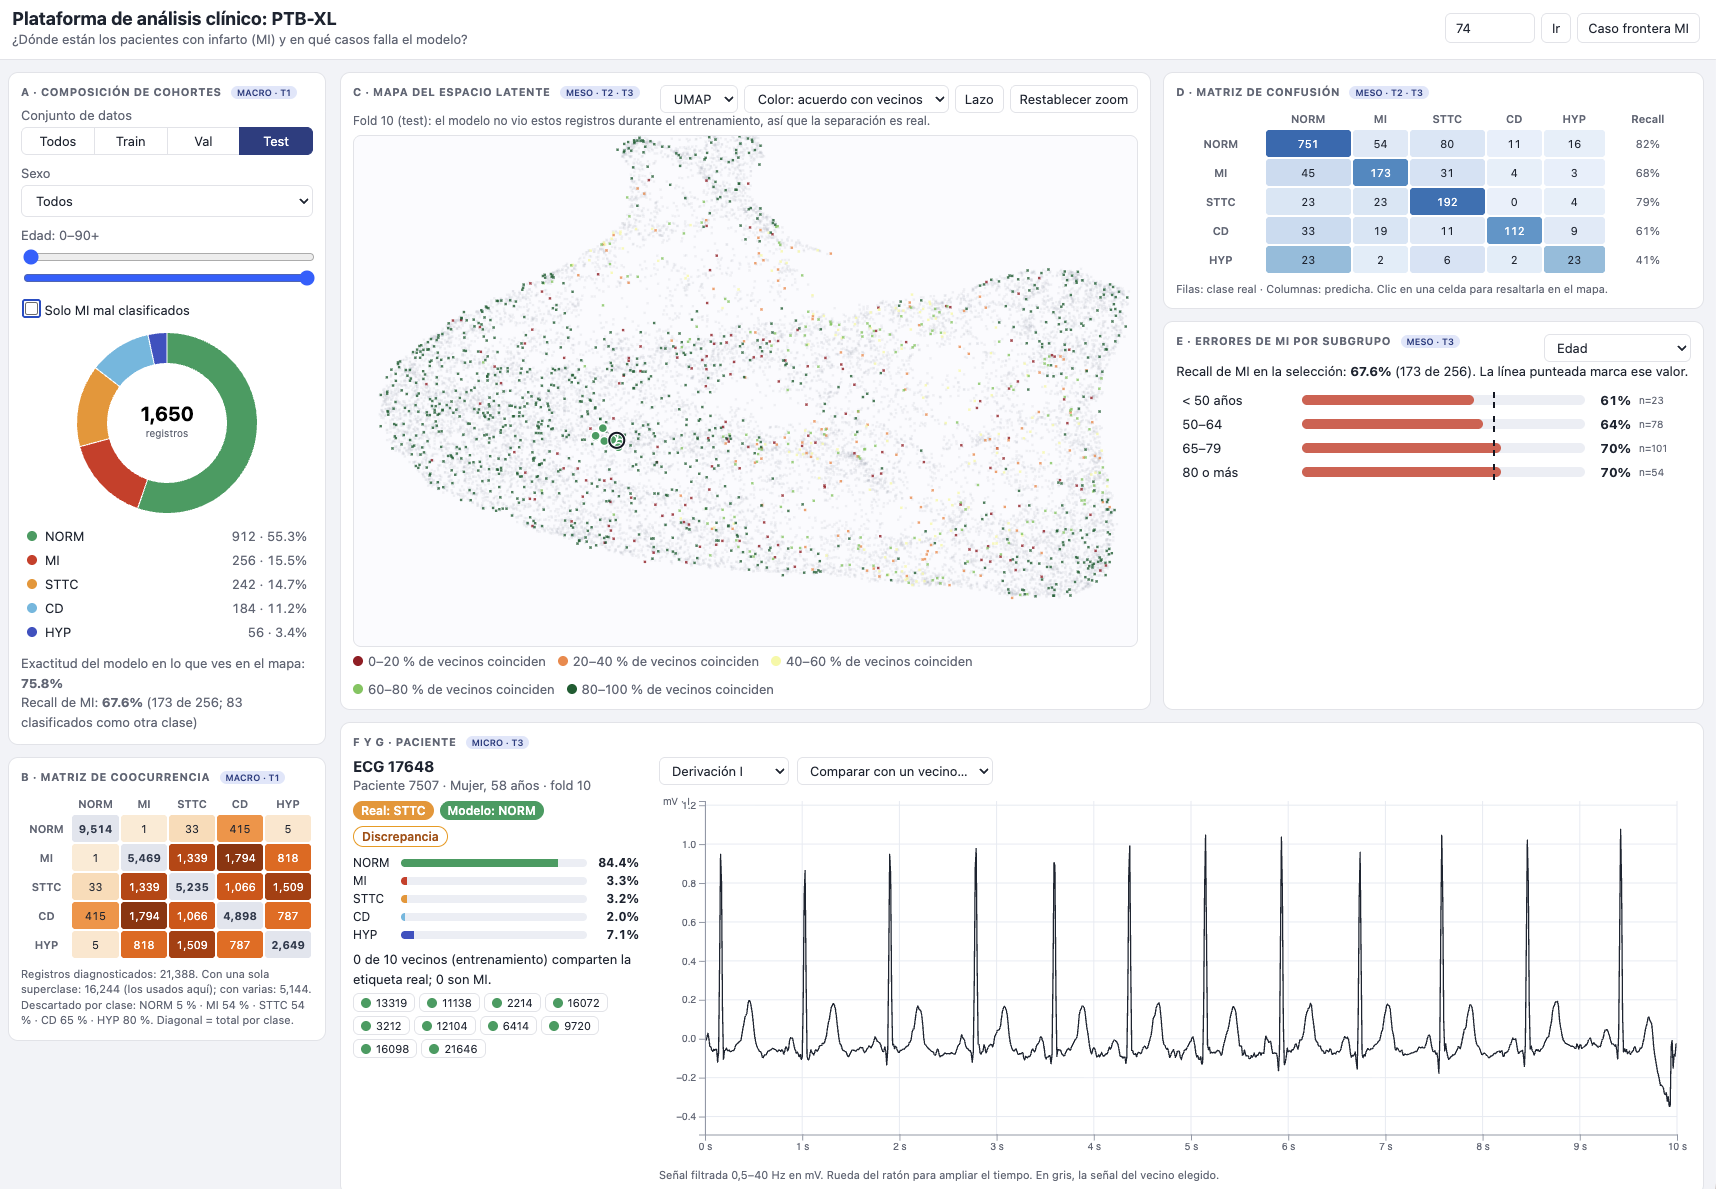
\includegraphics[width=0.95\textwidth]{figuras/plataforma_general.png}%
}{%
  \fbox{\parbox{0.8\textwidth}{\centering\small\textbf{Pendiente:} captura de la plataforma (conjunto de prueba, color por diagnóstico real) guardada como \texttt{figuras/plataforma\_general.png}.}}%
}
\caption{La plataforma en funcionamiento con los registros de prueba: cohortes y coocurrencia (izquierda), mapa, matriz de confusión y errores de infarto (arriba a la derecha) y ficha y señal del paciente (abajo).}
\label{fig:plataforma}
\end{figure*}

\subsection{Descripción de las vistas}
\noindent\textbf{A. Cohortes (nivel general).} \emph{Qué muestra:} un resumen de cuántos registros hay de cada diagnóstico en el grupo elegido, con la exactitud del modelo y el recall de infarto. \emph{Variables:} diagnóstico, conjunto de datos, sexo y edad. \emph{Gráfico:} anillo con leyenda y controles de filtro. \emph{Interacciones:} filtros por conjunto, sexo y rango de edad, y un clic en una clase para resaltarla; todo se refleja en las demás vistas. \emph{Tarea:} T1.

\smallskip\noindent\textbf{B. Matriz de coocurrencia (nivel general).} \emph{Qué muestra:} qué diagnósticos aparecen juntos en un mismo registro; explica por qué trabajamos con un solo diagnóstico por registro. \emph{Variables:} número de registros por cada par de diagnósticos (sobre los 21.388 registros diagnosticados). \emph{Gráfico:} mapa de calor de $5\times5$. \emph{Interacciones:} al pasar el cursor se ve el conteo y el porcentaje. \emph{Tarea:} T1.

\smallskip\noindent\textbf{C. Mapa del espacio latente (nivel intermedio).} \emph{Qué muestra:} dónde se ubican los infartos frente a los demás diagnósticos, usando los resúmenes que calcula el modelo. \emph{Variables:} coordenadas UMAP o t-SNE; color por diagnóstico real, por predicción o por cuántos vecinos comparten el diagnóstico. \emph{Gráfico:} nube de puntos dibujada en un \emph{canvas}; lo que queda fuera del filtro se ve tenue. \emph{Interacciones:} zoom y desplazamiento, información al pasar el cursor, clic para elegir un registro (se marcan sus vecinos), selección con un lazo y cambio entre UMAP y t-SNE. \emph{Tareas:} T2 y T3.

\smallskip\noindent\textbf{D. Matriz de confusión (nivel intermedio).} \emph{Qué muestra:} cuántos registros de cada diagnóstico real el modelo clasifica en cada clase. \emph{Variables:} clase real y clase predicha, con el recall por fila. \emph{Gráfico:} mapa de calor de $5\times5$ con los números anotados. \emph{Interacciones:} un clic en una celda resalta en el mapa esos registros (por ejemplo, infartos clasificados como STTC) y atenúa el resto. \emph{Tareas:} T2 y T3.

\smallskip\noindent\textbf{E. Errores de infarto por subgrupo (nivel intermedio).} \emph{Qué muestra:} qué proporción de infartos detecta el modelo en cada grupo de pacientes. \emph{Variables:} recall y tamaño del grupo según tipo de infarto, sexo, edad, ruido o etapa. \emph{Gráfico:} barras horizontales con el tamaño del grupo; los grupos con menos de 15 casos se marcan como solo indicativos. \emph{Interacciones:} información al pasar el cursor y clic en una barra para resaltar ese grupo en el mapa. \emph{Tarea:} T3.

\smallskip\noindent\textbf{F. Ficha del paciente y vecinos (nivel de detalle).} \emph{Qué muestra:} para un registro, su diagnóstico real, lo que predice el modelo y qué dicen sus vecinos. \emph{Variables:} diagnóstico real, predicción, probabilidades de las cinco clases, tipo y etapa del infarto, edad, sexo y 10 vecinos con su diagnóstico. \emph{Gráfico:} tarjeta con barras de probabilidad y lista de vecinos. \emph{Interacciones:} un clic en un vecino salta a ese registro y lo marca en el mapa. \emph{Tarea:} T3.

\smallskip\noindent\textbf{G. Señal ECG (nivel de detalle).} \emph{Qué muestra:} la señal del registro, para compararla con la de uno de sus vecinos. \emph{Variables:} voltaje (mV) frente al tiempo (0 a 10~s) en cada una de las 12 derivaciones. \emph{Gráfico:} línea con la señal; la del vecino aparece encima en morado. \emph{Interacciones:} elegir la derivación, ampliar el tiempo y elegir con qué vecino comparar. \emph{Tarea:} T3.

\smallskip\noindent\textbf{H. Comparación con los vecinos (ventana emergente, nivel de detalle).} \emph{Qué muestra:} el latido medio del caso (mediana de sus latidos alineados en el pico R) frente a la plantilla de sus 10 vecinos, y cada vecino en miniatura. \emph{Variables:} voltaje (mV) frente al tiempo desde el pico R, en cada derivación; diagnóstico, distancia y correlación del latido de cada vecino con el del caso. \emph{Gráfico:} líneas superpuestas con franjas donde el caso difiere de la plantilla en más del 20\,\% de la amplitud del latido, barras con la diferencia media por derivación y una cuadrícula de 10 miniaturas. \emph{Interacciones:} elegir la derivación (también con un clic en su barra), elegir con qué vecinos se calcula la plantilla (todos, solo los de otra clase o solo los de su misma clase; los que entran se resaltan en las tarjetas y el resto se atenúa) y añadir vecinos al gráfico grande, uno a uno o con un botón que dibuja todos los de la plantilla (cada vecino conserva su color; los que no forman la plantilla quedan desactivados). Las franjas señalan dónde difieren las señales; no indican qué usó el modelo (Fig.~\ref{fig:comparacion}). \emph{Tarea:} T3.

\smallskip\noindent\textbf{I. Patrón de los infartos perdidos (ventana emergente, nivel intermedio).} \emph{Qué muestra:} dónde, en la señal, se diferencian los infartos perdidos de los detectados. \emph{Variables:} desviación del latido medio de cada infarto de prueba respecto al latido normal típico, por derivación y por tiempo desde el pico R, promediada en cada grupo. \emph{Gráfico:} dos tarjetas con el porcentaje de infartos más parecidos al latido normal, barras agrupadas por derivación (perdidos frente a detectados), dos tarjetas por zona del infarto y, como detalle, los tres mapas de calor (perdidos, detectados y su diferencia). \emph{Interacciones:} apertura desde la barra superior y despliegue del mapa de calor. \emph{Tarea:} T3.

\smallskip\noindent\textbf{J. Pruebas de apoyo (ventana emergente, nivel intermedio).} \emph{Qué muestra:} los análisis con los que se descartaron otras explicaciones de por qué se pierden los infartos. \emph{Variables:} infartos detectados y vecinos en común según la distancia (coseno, euclidiana, Manhattan y Chebyshev) y el tamaño del vecindario; distancia media y acuerdo de etiqueta con los vecinos; grupos de K-means y DBSCAN de los 83 infartos perdidos; recall de la red y del kNN con cinco variantes de la señal de entrada. \emph{Gráfico:} cuatro pestañas con tablas y barras. \emph{Interacciones:} cambio de pestaña y un botón que lleva al mapa con el color por grupo de K-means y solo los infartos mal clasificados. Son resultados calculados fuera de la plataforma, sobre los registros de prueba, y se cargan aquí para consultarlos: no se recalculan al filtrar. \emph{Tarea:} T3.

\subsection{Relación entre vistas y tareas}
El Cuadro~\ref{tab:vistas} indica qué tareas apoya cada vista y cómo se interactúa con ella.

\begin{table*}[t]
\centering
\caption{Relación entre vistas, atributos, tareas e interacciones.}
\label{tab:vistas}
\small
\renewcommand{\arraystretch}{1.1}
\begin{tabular}{L{4.2cm} l L{5.2cm} ccc L{4cm}}
\toprule
Vista & Nivel & Atributos representados & T1 & T2 & T3 & Interacciones principales \\
\midrule
A. Cohortes & General & Superclase, conjunto, sexo, edad & \checkmark & & & Filtrado cruzado \\
B. Matriz de coocurrencia & General & Pares de superclases & \checkmark & & & \emph{Tooltip} \\
C. Mapa del espacio latente & Intermedio & Embedding 2D, etiqueta, predicción, acuerdo & & \checkmark & \checkmark & Zoom, lazo, selección, \emph{tooltip} \\
D. Matriz de confusión & Intermedio & Clase real y predicha & & \checkmark & \checkmark & Clic en celda (resalta) \\
E. Errores de MI por subgrupo & Intermedio & Subtipo, sexo, edad, ruido, etapa & & & \checkmark & Clic en barra (resalta) \\
F. Ficha y vecinos & Detalle & Probabilidades, vecinos, metadatos & & & \checkmark & Clic en vecino (enlace) \\
G. Señal ECG & Detalle & Voltaje, tiempo, derivación & & & \checkmark & Derivación, zoom temporal, vecino \\
H. Comparación con vecinos & Detalle & Latido medio, plantilla, diferencia por derivación & & & \checkmark & Derivación, plantilla, hasta 10 vecinos \\
I. Patrón de los perdidos & Intermedio & Desviación por derivación y tiempo & & & \checkmark & Apertura desde la barra superior \\
J. Pruebas de apoyo & Intermedio & Distancias, lejanía de vecinos, agrupamientos, preprocesamiento & & \checkmark & \checkmark & Pestañas; enlace al mapa \\
\bottomrule
\end{tabular}
\end{table*}

\subsection{Un ejemplo de uso}
Para ver cómo se conectan las vistas seguimos un caso de la Fig.~\ref{fig:plataforma}. Empezamos en las cohortes (A) con el conjunto de prueba: de los 1.650 registros, 256 son infartos (15,5\,\%). En la matriz de confusión (D) vemos que el modelo detecta 173 de ellos (recall de 67,6\,\%), clasifica 45 como normales y 31 como STTC; al hacer clic en una celda, esos registros se resaltan en el mapa (C). Al elegir un punto del mapa se abre la ficha (F) y la señal (G). En la captura aparece el ECG 17648, de una mujer de 58 años: su diagnóstico real es STTC, pero el modelo dice NORM con 84,4\,\% de confianza, y ninguno de sus 10 vecinos más parecidos comparte la etiqueta real. Es un desacuerdo que conviene revisar: puede ser un error del modelo o una etiqueta dudosa. Al superponer la señal de un vecino (G) se puede comparar la forma de las ondas; esa revisión corresponde a la persona especialista. El mismo recorrido sirve para los infartos mal clasificados, con el botón <<Caso frontera MI>> o activando <<Solo MI mal clasificados>>.

% =====================================================================
\section{Resultados}
\subsection{Resultados del modelo y del mapa}
Para leer los cuadros: el AUC macro y el F1 macro miden qué tan bien clasifica el modelo en promedio entre las cinco clases (más alto es mejor); la exactitud balanceada es el promedio del recall de cada clase; el ECE mide cuánto se parece la confianza del modelo a su acierto real (más bajo es mejor); y el silhouette y el kNN miden qué tan ordenado quedó el espacio de 64 números.

El Cuadro~\ref{tab:resultados} compara los tres sistemas. La red neuronal supera al método clásico en unos 0,05 de AUC macro (0,927 frente a 0,881), así que sí aporta. La parte contrastiva no mejora la clasificación (AUC macro de 0,924 frente a 0,927) y queda algo mejor calibrada (ECE de 0,042 frente a 0,053), pero ordena mejor el espacio de 64 números (silhouette de 0,263 frente a 0,196). Hay además una limitación importante: aunque el AUC macro supera 0,90, el modelo detecta cerca de dos de cada tres infartos (recall de 0,68). Si se exige que solo el 10\,\% de los no infartos se marque como infarto, detecta 75\,\% de los infartos; esa cifra solo supera 0,80 en STTC y, por poco, en CD.

\begin{table}[t]
\centering
\caption{Resultados en los 1.650 registros de prueba. AUC, F1, exactitud balanceada, silhouette y kNN: más alto es mejor; ECE: más bajo es mejor. Silhouette y kNN se miden sobre el espacio de 64 números.}
\label{tab:resultados}
\scriptsize
\setlength{\tabcolsep}{3pt}
\begin{tabular}{lcccccc}
\toprule
Modelo & AUC & F1 & Exact. & ECE & Silh. & kNN \\
 & macro & macro & balanc. & & & \\
\midrule
CNN, solo entropía cruzada & 0,927 & 0,671 & 0,711 & 0,053 & 0,196 & 0,790 \\
CNN, entropía cruzada + SupCon & 0,924 & 0,664 & 0,660 & 0,042 & 0,263 & 0,777 \\
Características + gradient boosting & 0,881 & 0,569 & 0,555 & 0,062 & -- & -- \\
\bottomrule
\end{tabular}
\end{table}

El Cuadro~\ref{tab:errores} resume dónde falla más el modelo con los infartos (489 en total, en validación y prueba, con un recall de 0,65). Los infartos anteriores, los de mujeres y los de etapa desconocida se detectan peor. Son diferencias exploratorias (prueba de dos proporciones): sirven para formular hipótesis, no para afirmar causas. El ruido de la señal no marca una diferencia clara. Tampoco podemos usar la validación humana de la etiqueta para estudiar etiquetas dudosas, porque los grupos 9 y 10 solo contienen registros validados.

\begin{table}[t]
\centering
\caption{Proporción de infartos que el modelo detecta en cada grupo (registros de validación y prueba). Un valor $p$ pequeño indica que la diferencia entre los dos grupos difícilmente es casualidad.}
\label{tab:errores}
\small
\begin{tabular}{llrcc}
\toprule
Variable & Grupo & $n$ & Recall & $p$ \\
\midrule
Subtipo & Anterior (AMI) & 160 & 0,56 & \multirow{2}{*}{$<0{,}001$} \\
        & Inferior (IMI) & 313 & 0,72 & \\
Sexo    & Hombre & 277 & 0,71 & \multirow{2}{*}{0,003} \\
        & Mujer  & 212 & 0,58 & \\
Etapa   & Conocida & 201 & 0,74 & \multirow{2}{*}{0,001} \\
        & Desconocida & 288 & 0,59 & \\
Ruido   & Sin ruido & 340 & 0,67 & \multirow{2}{*}{0,20} \\
        & Con ruido & 149 & 0,61 & \\
\bottomrule
\end{tabular}
\end{table}

\textbf{Evaluación del mapa 2D.} Para comprobar que el resumen aprendido mejora el mapa, dibujamos con UMAP la señal cruda, las 124 características y el resumen de la red con y sin pérdida contrastiva, y añadimos t-SNE sobre el resumen. Los mapas con UMAP se ajustan con los registros de entrenamiento y se evalúan sobre los de prueba (t-SNE, que no puede ubicar puntos nuevos, se calcula con todos los registros), con las medidas de la sección~III-D calculadas sobre las dos coordenadas del mapa. Hay que tener presente que el resumen de la red se entrena con las etiquetas y la señal cruda no; la comparación mide, por tanto, el valor de una representación aprendida. Los resultados están en el Cuadro~\ref{tab:proyecciones} y en la Fig.~\ref{fig:proyecciones}, y se discuten en la sección~VII.

\IfFileExists{tabla_proyecciones.tex}{%
  \begin{table}[t]
\centering
\caption{Métricas sobre el mapa 2D (fold de test). En negrita, el mejor valor de cada columna.}
\label{tab:proyecciones}
\scriptsize
\setlength{\tabcolsep}{3pt}
\begin{tabular}{lccccc}
\toprule
Proyección & kNN & Silh. & Recall MI & AUC MI & Trust. \\
\midrule
Señal cruda + UMAP & 0,527 & -0,072 & 0,047 & 0,543 & 0,668 \\
Características + UMAP & 0,588 & -0,067 & 0,191 & 0,695 & 0,834 \\
Embedding solo CE + UMAP & \textbf{0,785} & 0,071 & \textbf{0,578} & 0,890 & 0,949 \\
Embedding CE+SupCon + UMAP & 0,772 & \textbf{0,077} & 0,570 & \textbf{0,896} & 0,969 \\
Embedding CE+SupCon + t-SNE & 0,775 & 0,034 & 0,559 & 0,893 & \textbf{0,986} \\
\bottomrule
\end{tabular}
\end{table}
%
}{%
  \par\smallskip\noindent\fbox{\parbox{0.95\columnwidth}{\small\textbf{Pendiente:} ejecutar la sección 12 del notebook v3.1 y generar \texttt{tabla\_proyecciones.tex} con \texttt{csv\_a\_latex.py}.}}\par\smallskip
}

\begin{figure*}[t]
\centering
\IfFileExists{figuras/comparacion_proyecciones.png}{%
  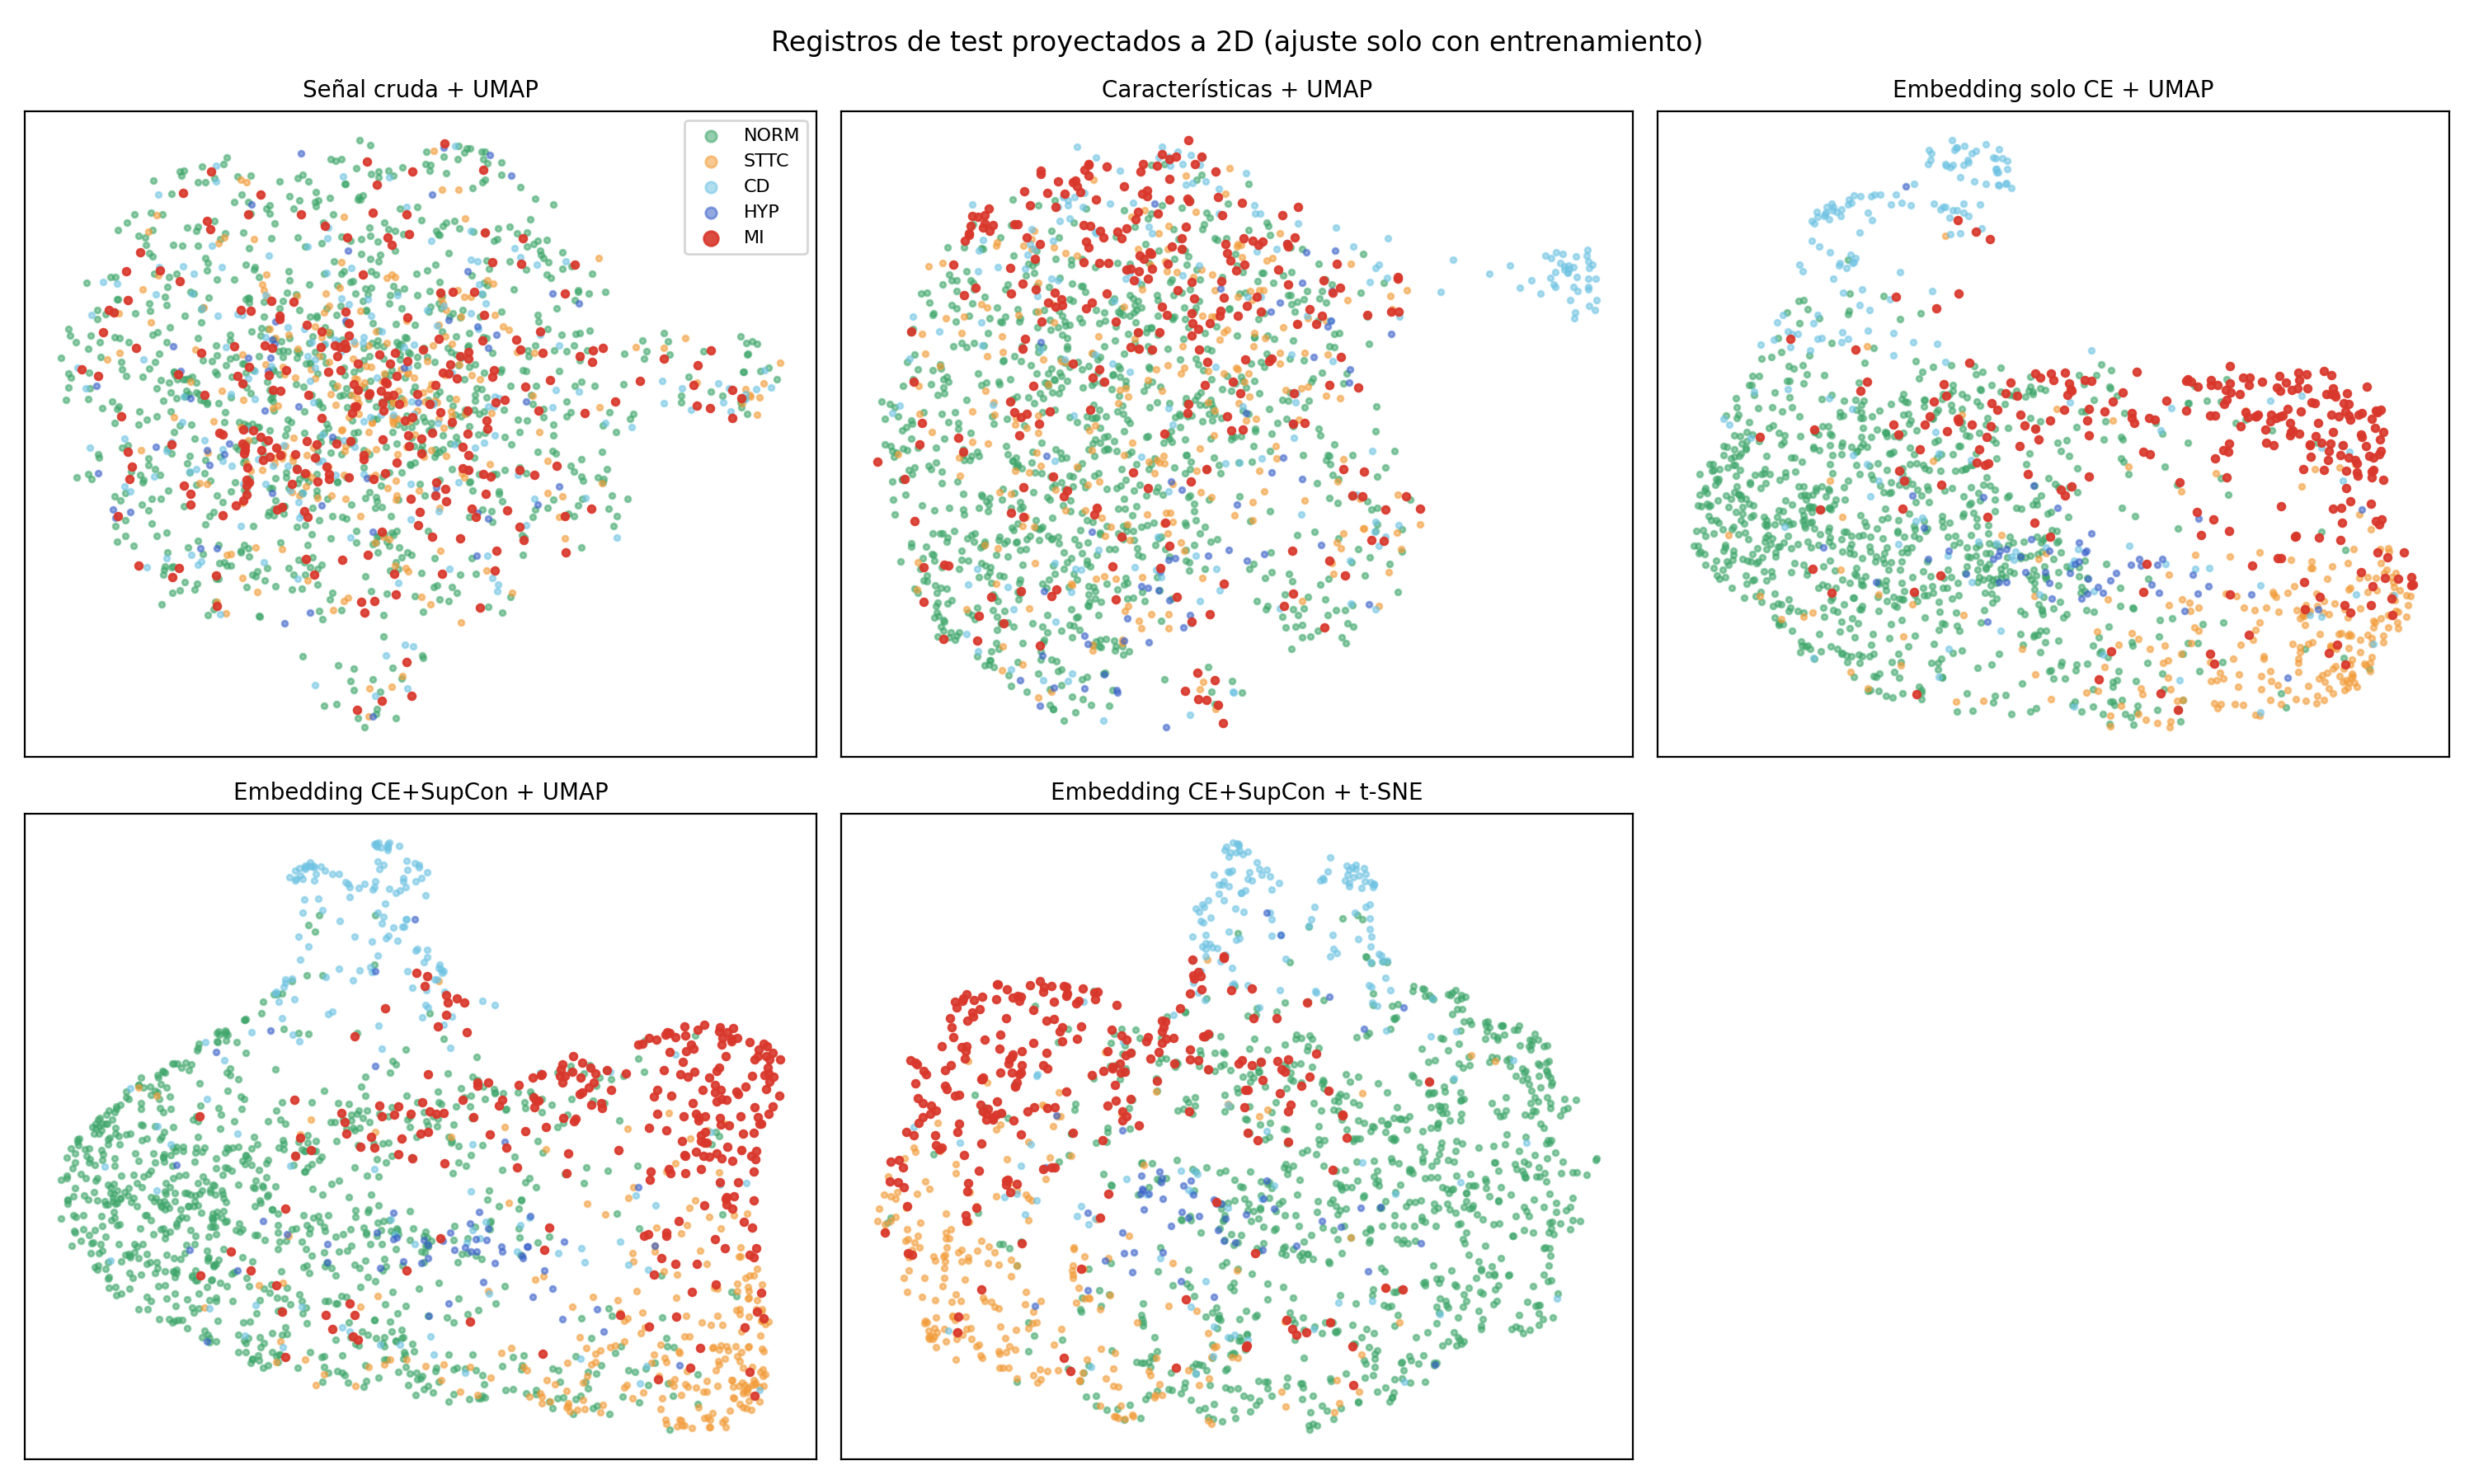
\includegraphics[width=0.85\textwidth]{figuras/comparacion_proyecciones.png}%
}{%
  \fbox{\parbox{0.8\textwidth}{\centering\small\textbf{Pendiente:} copiar \texttt{comparacion\_proyecciones.png} (lo genera el notebook v3.1) a la carpeta \texttt{figuras/}.}}%
}
\caption{Registros de prueba proyectados a 2D con distintas representaciones (UMAP ajustado solo con entrenamiento; t-SNE calculado con todos los registros). MI se dibuja al final, en rojo.}
\label{fig:proyecciones}
\end{figure*}

\subsection{Vecinos, distancias y agrupamientos}
Para entender por qué fallan los infartos mal clasificados revisamos tres cosas sobre los 1.650 registros de prueba: si el resultado depende de la distancia usada para buscar vecinos, qué tan lejos están esos vecinos y si los algoritmos de agrupamiento separan a los infartos. Recalculamos los resúmenes con el modelo guardado y comprobamos que sus predicciones coinciden con las de la plataforma en el 100\,\% de los registros. Las clases de los vecinos se toman de los registros de entrenamiento y usamos $K=10$.

\subsubsection{Efecto de la distancia}
Comparamos la distancia coseno, la euclidiana, la de Manhattan y la de Chebyshev sobre los 64 números, y tres de ellas sobre los 128 números previos a la proyección. Con el voto de los 10 vecinos medimos cuántos infartos se reconocen (Cuadro~\ref{tab:metricas}). La red neuronal, que es la que clasifica en la plataforma, queda como referencia.

\begin{table}[t]
\caption{Voto de 10 vecinos según la distancia (prueba, $n=1.650$). Jaccard: parecido de los conjuntos de vecinos con los de coseno sobre 64 números.}
\label{tab:metricas}
\centering\footnotesize\setlength{\tabcolsep}{3pt}
\begin{tabular}{@{}lccc@{}}
\toprule
Clasificador & Exactitud & Recall MI & Jaccard \\
\midrule
Red (plataforma) & 0,758 & 0,676 & -- \\
kNN 64, cos. = eucl. & 0,776 & 0,598 & 1,00 \\
kNN 64, Manhattan & 0,778 & 0,609 & 0,82 \\
kNN 64, Chebyshev & 0,772 & 0,570 & 0,53 \\
kNN 128, cos. & 0,785 & 0,617 & 0,30 \\
kNN 128, eucl. & 0,778 & 0,566 & 0,25 \\
kNN 128, Manh. & 0,783 & 0,563 & 0,26 \\
\bottomrule
\end{tabular}
\end{table}

El coseno y la euclidiana dan exactamente los mismos vecinos porque el resumen de 64 números está normalizado. Cambiar de coseno a Manhattan modifica la predicción de solo 3 de los 256 infartos, y a Chebyshev la de 14. Aunque los vecinos cambian bastante (hasta compartir solo 25\,\% en el espacio de 128 números), el recall de infartos se mueve apenas entre 0,56 y 0,62. En ningún caso el kNN supera a la red en infartos. De los 83 infartos que la red no detecta, el kNN con coseno solo acierta 3; y falla en 23 de los 173 que la red sí detecta. La fila de infartos de la matriz de confusión del kNN ($K=10$) es: 153 bien clasificados, 68 como NORM, 25 como STTC, 8 como CD y 2 como HYP; la de la red es 173, 45, 31, 4 y 3. También variamos $K$ (1, 3, 5, 10, 20 y 50) con coseno sobre los 64 números: la exactitud sube de 0,72 a 0,78 y el recall de infartos se mueve solo entre 0,56 y 0,60, con su valor más alto en $K=10$. Es decir, ni el tamaño del vecindario rescata a los infartos que fallan.

\subsubsection{Distancia a los vecinos}
Un vecino siempre existe, aunque esté lejos. Por eso medimos la distancia coseno a los 10 vecinos (Cuadro~\ref{tab:vecinos}). Las distancias absolutas son muy pequeñas en todos los registros, así que solo sirven para comparar. Los infartos mal clasificados tienen vecinos alrededor de 30\,\% más lejos que los bien clasificados, y solo 13\,\% de sus vecinos comparten la etiqueta real (índice $\kappa$ de 0,13), frente a 76\,\% en los infartos bien clasificados. El voto de esos vecinos es NORM en 48 casos y STTC en 25 de los 83: caen dentro de zonas que el modelo asocia con otras clases.

\begin{table}[t]
\caption{Distancia a los vecinos y acuerdo con la etiqueta real (prueba).}
\label{tab:vecinos}
\centering\footnotesize\setlength{\tabcolsep}{3pt}
\begin{tabular}{@{}lccc@{}}
\toprule
Grupo & $n$ & Dist. ($\times10^{-3}$) & $\kappa$ medio \\
\midrule
MI bien clasificados & 173 & 2,83 & 0,76 \\
MI mal clasificados & 83 & 3,69 & 0,13 \\
Otras clases & 1.394 & 3,03 & -- \\
\bottomrule
\end{tabular}
\end{table}

\subsubsection{Agrupamientos}
Ajustamos K-means ($k=5$) y DBSCAN (distancia coseno, mínimo 10 puntos) con los registros de entrenamiento y asignamos los de prueba. K-means obtuvo una pureza de 0,74 (ARI de 0,41). Un grupo reúne 176 de los 256 infartos y contiene a 172 de los 173 infartos bien clasificados. En cambio, 79 de los 83 infartos mal clasificados caen en grupos dominados por otra clase (44 en NORM, 30 en STTC y 5 en CD). DBSCAN no fue informativo: con el valor de $\varepsilon$ que dejaba menos del 20\,\% de ruido, el 80\,\% de los registros cae en un solo grupo (ARI de 0,001). Probamos solo tres valores de $\varepsilon$, por lo que este resultado muestra que los infartos no forman un grupo aislado y denso, pero no descarta otros ajustes.

\subsubsection{Preprocesamiento, etiqueta y forma de la señal}
Para descartar otras explicaciones del error revisamos tres posibles causas, todas con los 256 infartos de prueba (173 detectados y 83 perdidos): el preprocesamiento de la señal, la calidad de la etiqueta y la forma de la señal.

\textbf{Preprocesamiento.} No reentrenamos con otro preprocesamiento. En su lugar, cambiamos la señal de entrada de la red ya entrenada con cinco variantes: un filtro pasa-bajas a 25~Hz, un pasa-altas a 1~Hz, ruido gaussiano, y amplitud multiplicada por 0,8 y por 1,2. El recall de infarto de la red quedó entre 0,668 y 0,688 (0,676 sin cambio). Entre 2 y 8 de los 83 infartos perdidos pasan a detectarse y entre 2 y 9 de los 173 detectados se pierden; el kNN se mueve en un rango similar (recall entre 0,555 y 0,605). Es decir, los infartos perdidos no desaparecen con estos cambios. Esto mide cuánto depende el resultado de la entrada, no lo que pasaría si se entrenara con otro preprocesamiento.

\textbf{Etiqueta y calidad del registro.} Los 256 infartos de prueba figuran como validados por una persona en PTB-XL, así que esa variable no distingue a los perdidos. El ruido anotado es algo más frecuente en los perdidos (29 de 83, 35\,\%, frente a 47 de 173, 27\,\%), sin diferencia clara (prueba exacta de Fisher, $p=0{,}24$). La etapa desconocida sí lo es (55 de 83, 66\,\%, frente a 91 de 173, 53\,\%; $p=0{,}044$), lo que coincide con lo ya visto por subgrupo; es una diferencia exploratoria. De los 83 perdidos, 23 tienen más de 70\,\% de probabilidad de NORM y a lo sumo un vecino de su clase; son candidatos para que un especialista revise si el ECG es sutil o la etiqueta es discutible. No podemos separar ambas cosas con estos datos.

\textbf{Forma de la señal.} Para comparar un caso con sus vecinos sin depender de una sola derivación ni de la posición de cada latido, calculamos el latido medio de cada registro (mediana de los latidos alineados en el pico R, en las 12 derivaciones) y su correlación con el de otro registro. Para los 256 infartos, la mediana de la correlación con el vecino más cercano es de 0,68, con el décimo vecino de 0,62 y con registros al azar de 0,52 (la correlación al azar no es cero porque todos los latidos comparten una forma general). En el 88\,\% de los casos, el vecino más cercano se parece más al caso que el promedio de registros al azar. Los vecinos se parecen entonces más que al azar, pero no son iguales. Los vecinos de los infartos perdidos, que son de otra clase, también se parecen a ellos (0,74): su latido medio es parecido al de registros que no son infarto, lo que es coherente con que la red los confunda.

\subsubsection{Dónde se diferencian los infartos perdidos en la señal}
Para ver si los infartos perdidos dejan una huella en la señal, comparamos el latido medio de cada uno de los 256 infartos de prueba (construido como antes, alineado en el pico R) con dos referencias de entrenamiento: el latido medio típico de registros normales y el de infartos, cada uno la mediana de 1\,500 registros al azar. La desviación es la diferencia absoluta dividida por la amplitud del latido de esa derivación (con un mínimo de 0,2~mV), promediada por derivación y por instante (Fig.~\ref{fig:patron}).

\begin{figure*}[t]
\centering
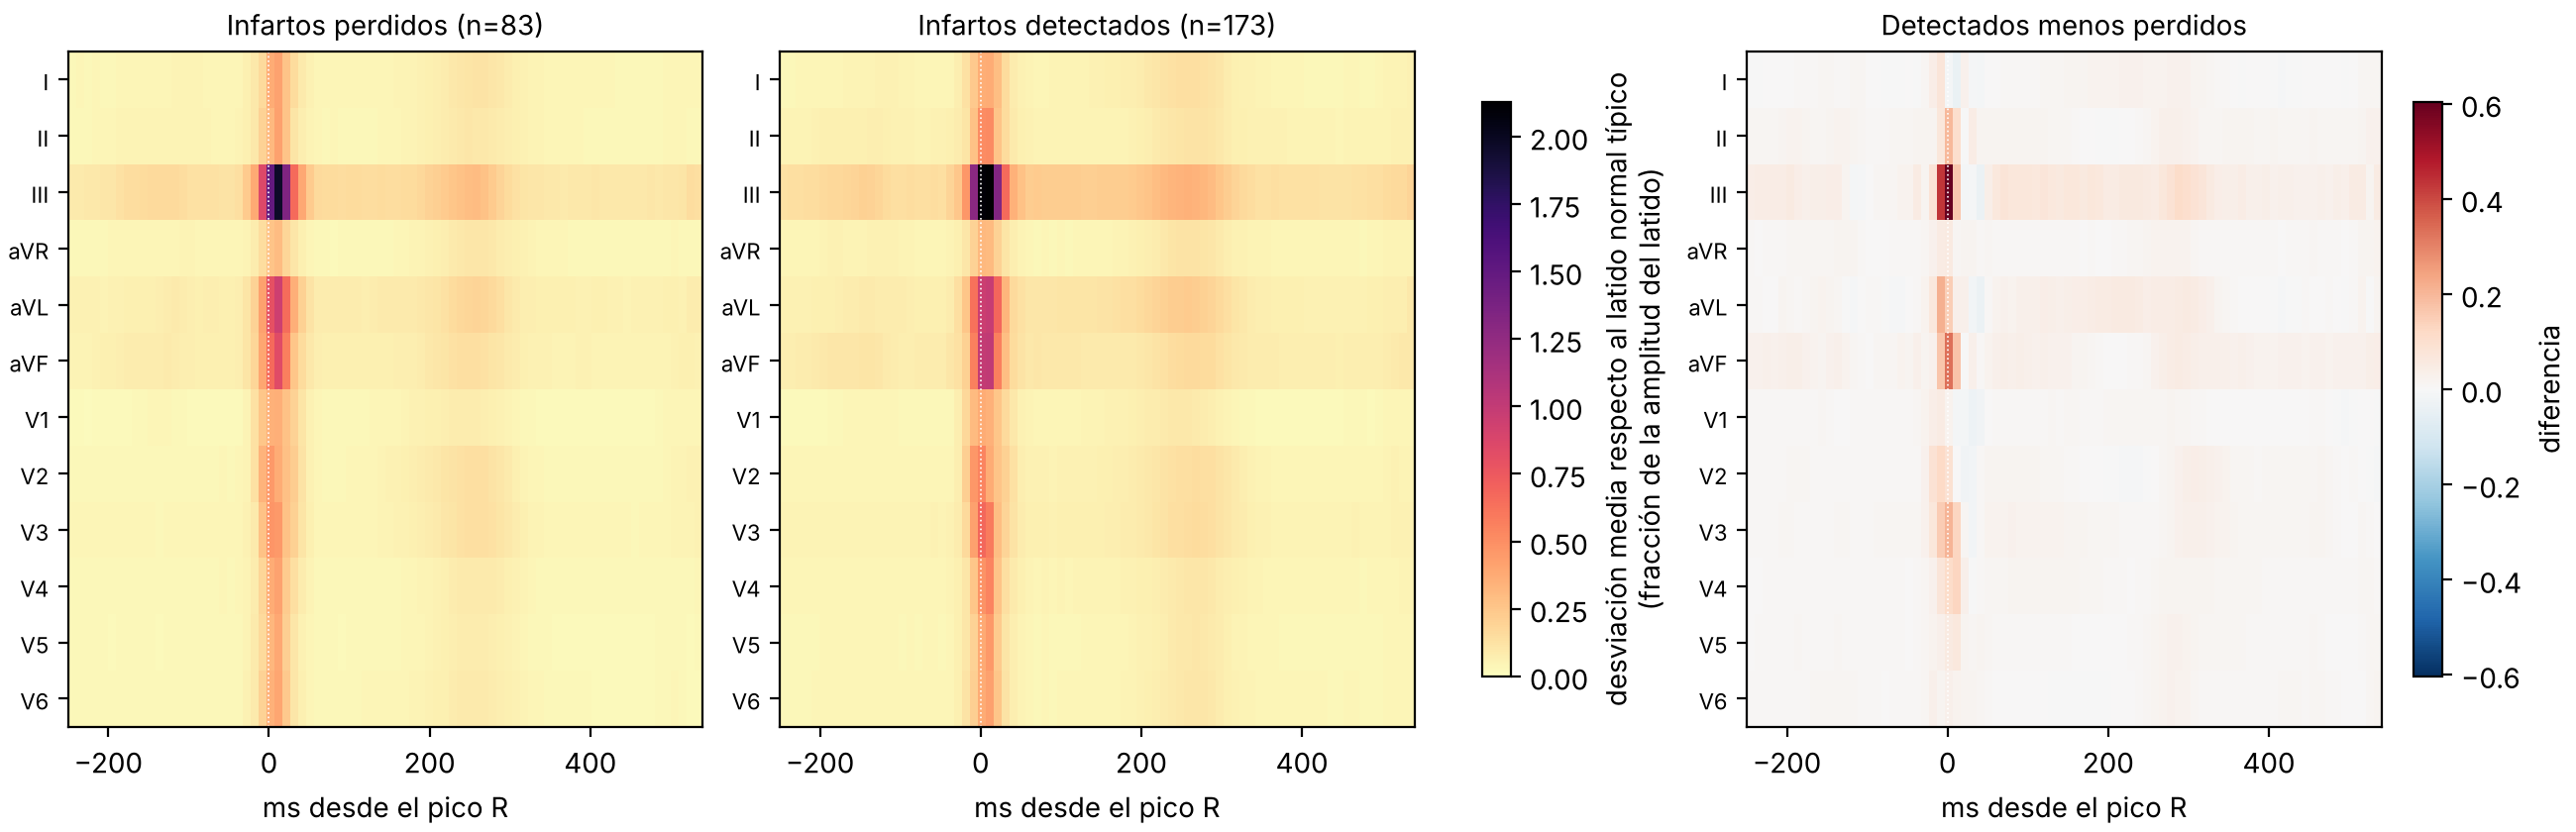
\includegraphics[width=0.95\textwidth]{figuras/patron_mapa.png}
\caption{Desviación media respecto al latido normal típico, por derivación y por tiempo desde el pico R, para los 83 infartos perdidos, los 173 detectados y su diferencia (detectados menos perdidos). Registros de prueba.}
\label{fig:patron}
\end{figure*}

\textbf{Respecto al latido normal.} Los infartos perdidos se desvían menos que los detectados en casi todas las derivaciones (prueba de Mann--Whitney con corrección de Benjamini--Hochberg: significativo en 11 de 12; la excepción es la derivación I, $p=0{,}077$). La diferencia se concentra en el complejo QRS de las derivaciones III, aVF y aVL (la desviación media del QRS es 0,25 en los perdidos y 0,29 en los detectados) y es pequeña en el segmento ST (0,05 contra 0,07) y la onda T (0,06 contra 0,08).

\textbf{Por zona del infarto.} En el conjunto de prueba, los infartos inferiores se detectan más (125 de 167, 75\,\%) que los anteriores (47 de 85, 55\,\%; Fisher, $p=0{,}003$); el Cuadro~\ref{tab:errores}, que junta validación y prueba, da 0,72 y 0,56. Dentro de cada tipo, la desviación respecto al latido normal en las derivaciones donde se espera la huella es menor en los perdidos: en los inferiores (II, III, aVF) 0,13 contra 0,17 ($p<0{,}001$) y en los anteriores (V1 a V4) 0,07 contra 0,09 ($p=0{,}011$). Los infartos laterales (4) son pocos para analizarlos.

\textbf{Parecido con las dos referencias.} La correlación del latido medio con el normal típico y con el infarto típico es 0,67 y 0,74 en los detectados (solo el 18\,\% queda más cerca del normal) y 0,78 y 0,77 en los perdidos (el 43\,\% queda más cerca del normal; $p<10^{-8}$ en la diferencia entre ambos grupos). Frente al latido de infarto típico, los perdidos no se distinguen de los detectados en ninguna derivación (valores $p$ corregidos desde 0,23).

\textbf{Cómo leerlo.} Los infartos perdidos no son registros ``raros'': se parecen al infarto típico tanto como los detectados, pero su huella respecto al ECG normal es más débil, en las mismas derivaciones donde los detectados la tienen más marcada. Hay tres cautelas. Primero, que la red detecte justo los que más se desvían del normal es en parte esperable, así que esto describe el error más que lo explica. Segundo, la desviación en el QRS depende de la alineación y del ancho del complejo, no solo de su amplitud. Tercero, es un solo entrenamiento y 256 infartos, sin validación clínica; no sabemos si una desviación menor corresponde a un infarto sutil o a una etiqueta discutible.

\subsubsection{Lectura conjunta}
Las tres revisiones apuntan a lo mismo: los infartos mal clasificados no son un problema de la distancia ni del algoritmo de vecinos. Sus vecinos son de otra clase, están algo más lejos y quedan dentro de los grupos normales o STTC del espacio que aprendió la red. Los infartos perdidos conservan la forma general de un infarto, pero su huella frente al ECG normal es más débil en las derivaciones donde se espera, sobre todo en el QRS. Los cambios de preprocesamiento de la entrada no hacen desaparecer estos errores, pero no reentrenamos con otro preprocesamiento ni separamos un error del modelo de una etiqueta dudosa.

\subsection{Estudio de casos}
Como no contamos con expertos externos, los autores actuamos como usuarios de la plataforma: la usamos para responder las tres tareas (T1 a T3) y describimos qué conocimiento obtuvimos en cada vista. El Cuadro~\ref{tab:tareas} resume ese recorrido (la plataforma se muestra en la Fig.~\ref{fig:interfaz} y, con los infartos perdidos resaltados, en la Fig.~\ref{fig:perdidos}), y a continuación detallamos la tarea T3 con tres infartos concretos.

\begin{table*}[t]
\caption{Recorrido por las tareas: qué hicimos en la plataforma y qué conocimiento obtuvimos (conjunto de prueba, salvo que se indique otra cosa).}
\label{tab:tareas}
\centering\footnotesize
\renewcommand{\arraystretch}{1.15}
\begin{tabularx}{\textwidth}{@{}>{\raggedright\arraybackslash}p{2.7cm}>{\raggedright\arraybackslash}p{1.5cm}>{\raggedright\arraybackslash}p{4.8cm}>{\raggedright\arraybackslash}X@{}}
\toprule
Tarea & Vistas & Qué hicimos & Conocimiento obtenido \\
\midrule
T1. Explorar cohortes & A, B &
Elegimos el conjunto Test y filtramos por sexo y edad; leímos la composición en el anillo y la coocurrencia de diagnósticos. &
El conjunto de prueba tiene 1.650 registros y 256 infartos (15,5\,\%). Un infarto casi nunca aparece junto a un registro normal (1 caso), pero sí junto a trastornos de conducción (1.794) y cambios ST-T (1.339); por eso trabajamos con un solo diagnóstico por registro. \\
T2. Comprobar si los infartos se agrupan & C, D &
Coloreamos el mapa por diagnóstico real y por acuerdo con los vecinos, y comparamos con la matriz de confusión. &
Los infartos forman una región reconocible pero no aislada: con dos coordenadas se recupera cerca del 57\,\% (frente a 5\,\% con la señal cruda). La red detecta 173 de 256 (recall 0,68); 45 pasan a NORM y 31 a STTC (Fig.~\ref{fig:perdidos}). \\
T3. Revisar los casos frontera & E, F, G, H, I, J &
Resaltamos los infartos perdidos, miramos el recall por subgrupo, abrimos casos con sus 10 vecinos y comparamos su latido con el de la plantilla de vecinos. &
Los perdidos se detectan peor en infartos anteriores (55\,\% frente a 75\,\%), mujeres y etapa desconocida. Sus vecinos son de otra clase (13\,\% de acuerdo frente a 76\,\%) y están más lejos; en la señal conservan la forma del infarto, con menor desviación del latido normal en el QRS de III, aVF y aVL. Los tres casos siguientes lo ilustran. \\
\bottomrule
\end{tabularx}
\end{table*}

\begin{figure*}[t]
\centering
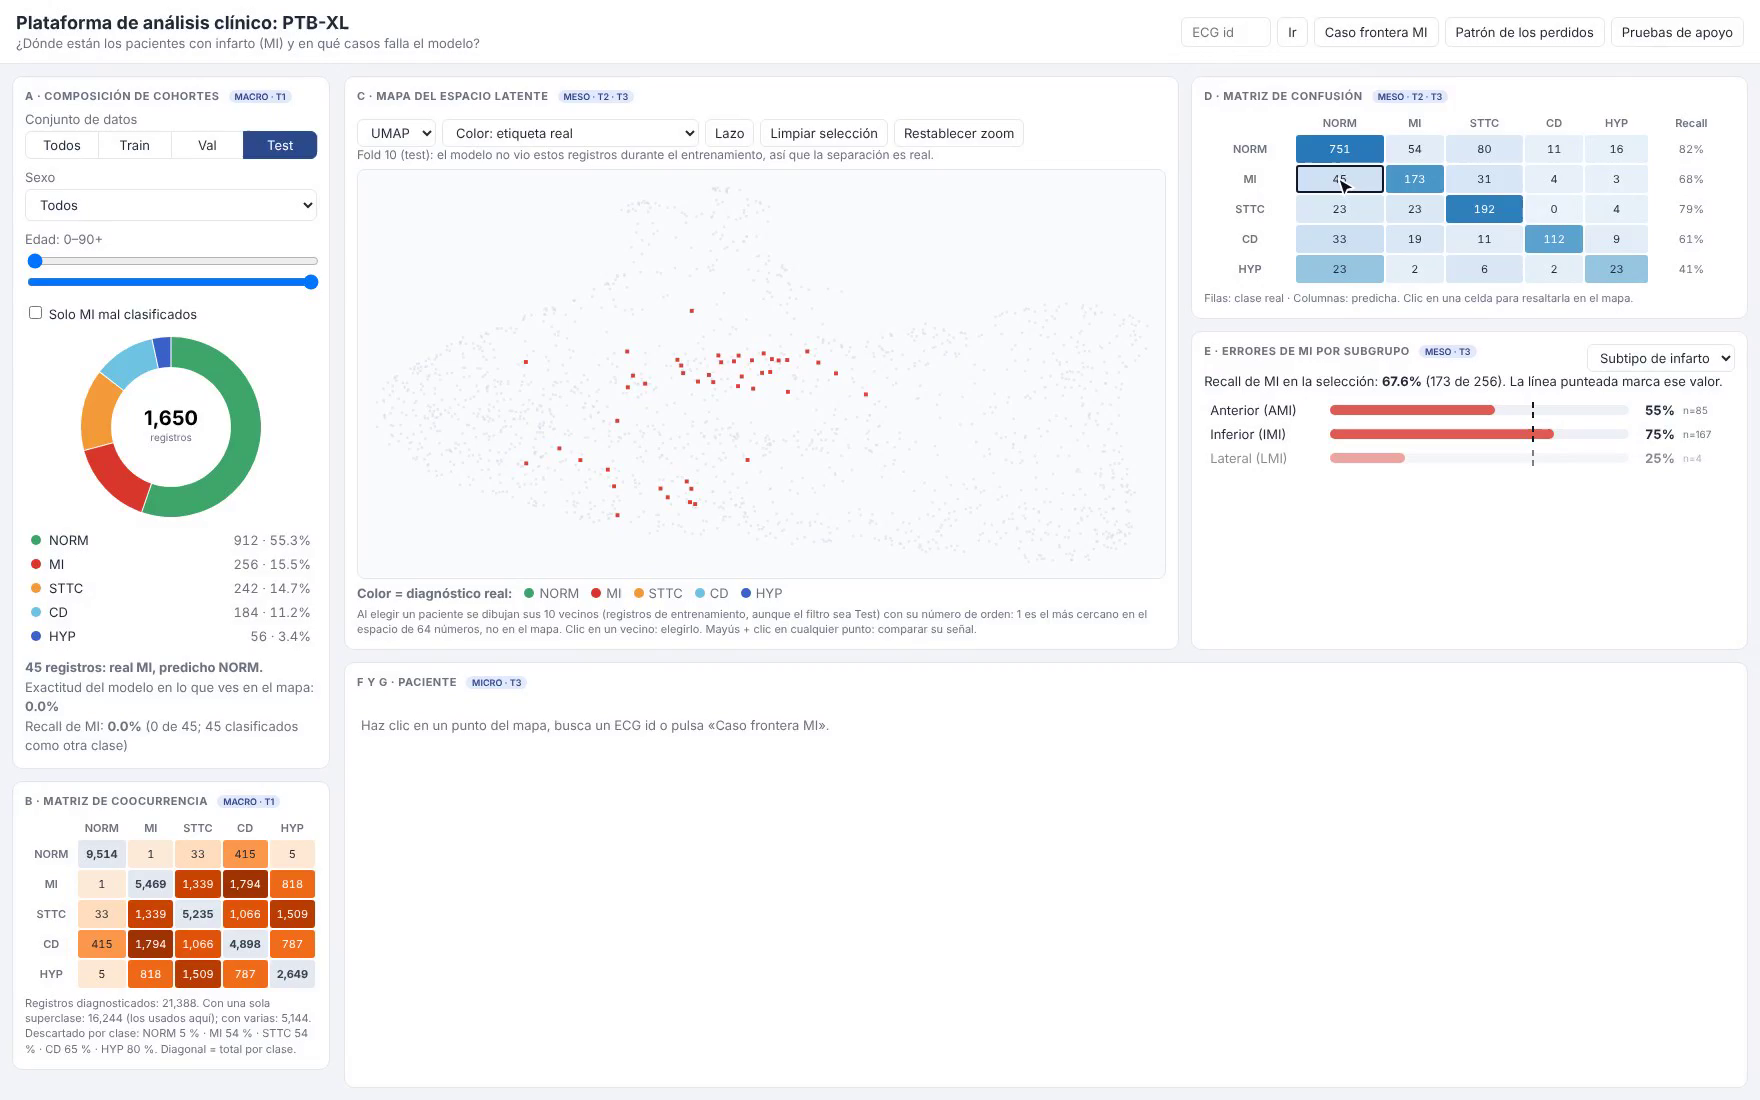
\includegraphics[width=0.8\textwidth]{figuras/plataforma_perdidos.png}
\caption{Plataforma con el conjunto de prueba y un clic en la celda MI $\to$ NORM de la matriz de confusión (vista D): el mapa (vista C) resalta en rojo los 45 infartos que la red clasifica como normales, dispersos por el mapa. La vista E muestra el recall por tipo de infarto de toda la selección.}
\label{fig:perdidos}
\end{figure*}

Para ver con ejemplos lo que muestran los números anteriores, seguimos tres infartos de prueba (Cuadro~\ref{tab:casos} y Fig.~\ref{fig:casos}). Los elegimos para cubrir tres situaciones: un acierto claro, un error en el que la red y los vecinos coinciden, y un caso en que no coinciden. Son ejemplos ilustrativos y no una muestra representativa. En la figura superponemos, en una derivación, la señal del caso con la de su vecino más cercano y con la de su décimo vecino. No interpretamos clínicamente las formas de onda: solo describimos lo que se ve en la comparación.

\begin{table*}[t]
\caption{Tres casos de infarto del conjunto de prueba. Distancia: coseno a los 10 vecinos (del más cercano al décimo). Sexo y edad según PTB-XL.}
\label{tab:casos}
\centering\footnotesize
\begin{tabular}{@{}lccc@{}}
\toprule
 & A. ECG 13078 & B. ECG 12137 & C. ECG 12991 \\
\midrule
Paciente & hombre, 67 años & mujer, 84 años & hombre, 84 años \\
Diagnóstico real & infarto inferior (IMI) & infarto anterior (AMI) & infarto anteroseptal (ASMI) \\
Etapa del infarto & II--III & desconocida & desconocida \\
Predicción de la red & MI (99,9\,\%) & NORM (78,6\,\%; MI 7,3\,\%) & STTC (48,1\,\%; MI 46,6\,\%) \\
Voto de los 10 vecinos & 10 MI & 10 NORM & 6 MI y 4 STTC \\
Distancias de los vecinos ($\times10^{-3}$) & 0,4 a 0,7 & 1,6 a 3,1 & 1,1 a 3,4 \\
kNN (coseno, Manhattan, Chebyshev) & MI & NORM & MI \\
Grupo de K-means & dominado por MI & dominado por NORM & dominado por MI \\
\bottomrule
\end{tabular}
\end{table*}

\begin{figure*}[t]
\centering
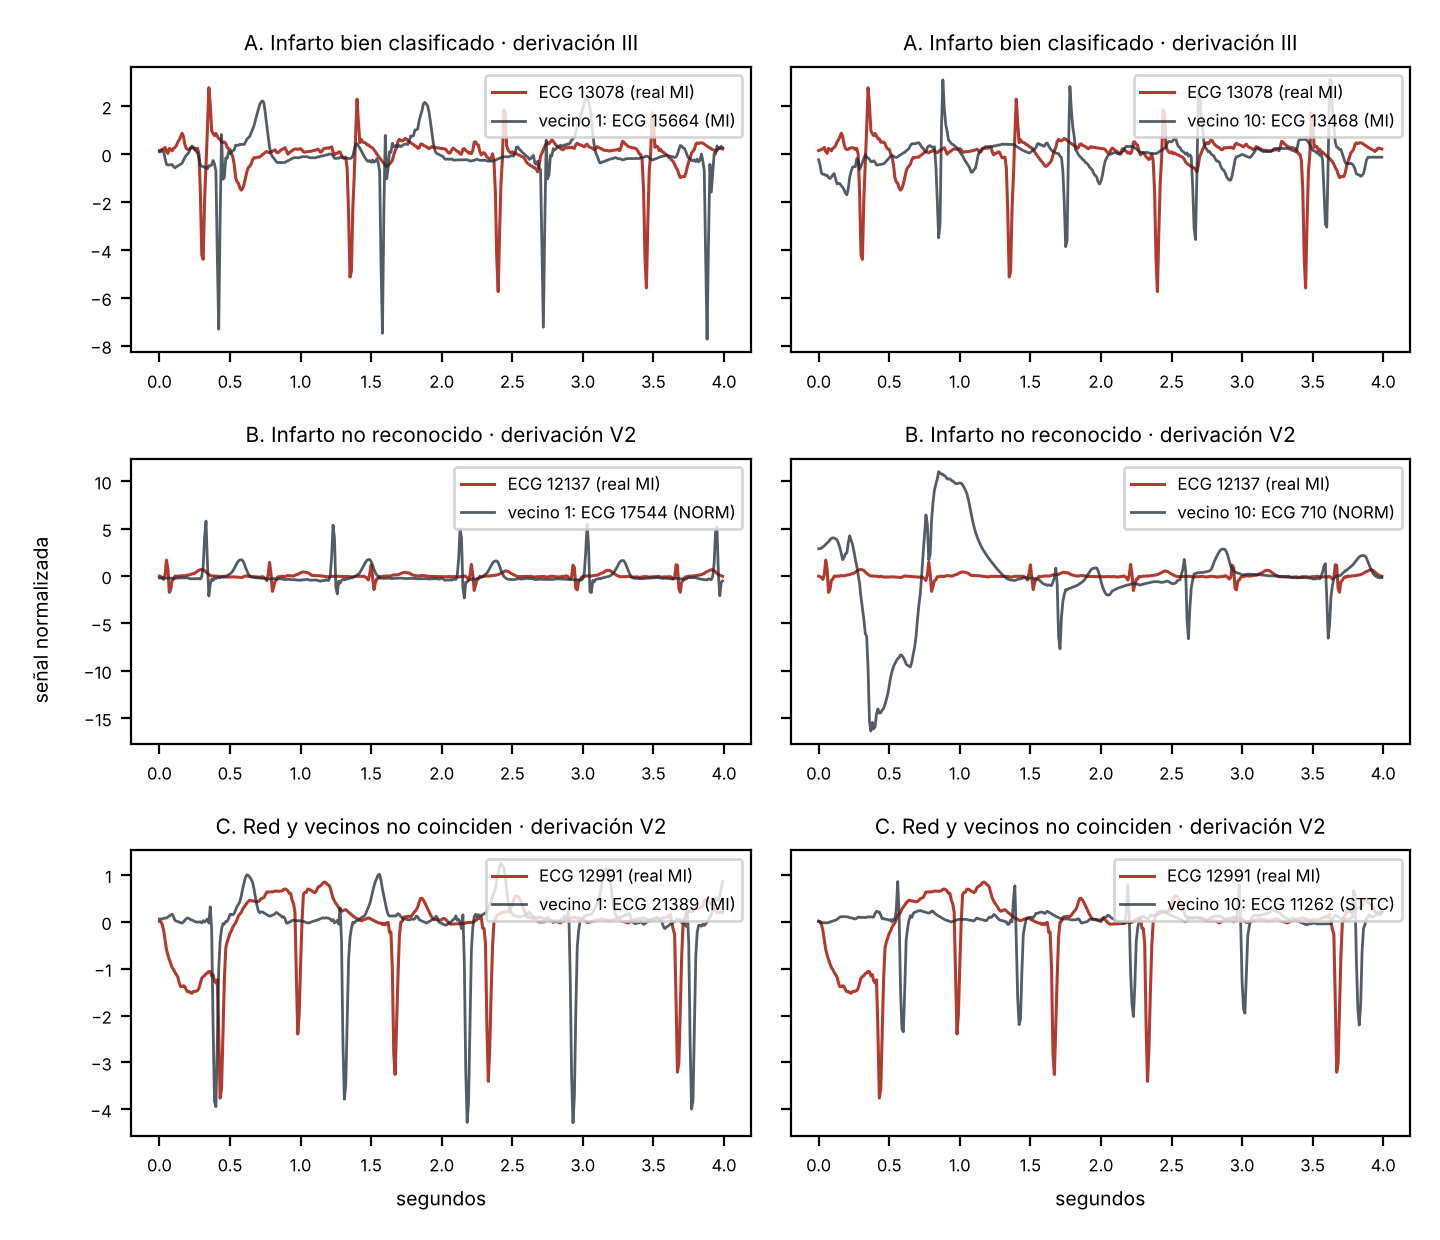
\includegraphics[width=0.8\textwidth]{figuras/casos_series.png}
\caption{Señal del caso (rojo) superpuesta a la de su vecino más cercano (izquierda) y a la de su décimo vecino (derecha), en una derivación y en los primeros 4 s. A: derivación III. B y C: derivación V2.}
\label{fig:casos}
\end{figure*}

\textbf{Caso A, acierto claro (ECG 13078).} La red da 99,9\,\% a infarto y los 10 vecinos son infartos, a distancias unas cuatro a siete veces menores que el promedio de los demás registros. Es lo que se espera de un caso bien ubicado: el modelo, los vecinos y el grupo de K-means coinciden. En la derivación III, el caso y sus vecinos tienen en común una deflexión negativa profunda en cada latido, aunque difieren en la amplitud y en el instante de cada latido.

\textbf{Caso B, error en el que todos coinciden (ECG 12137).} Es un infarto anterior de etapa desconocida que la red clasifica como normal. Sus 10 vecinos son normales y el kNN con las tres distancias también dice NORM. Importa que sus vecinos \emph{no} están lejos (distancia media de 2,8$\times10^{-3}$, similar a la de los registros normales): no es un caso de vecino ``forzado'', sino un registro que el modelo ubica entre normales. En V2, su señal tiene mucha menos amplitud que la de sus vecinos, y el décimo vecino tiene una oscilación lenta de gran amplitud al inicio que no está en el caso. Con estos datos no podemos decir si el infarto es sutil en el ECG o si la etiqueta es discutible; la etiqueta figura como validada por una persona en PTB-XL, y la lectura de la señal corresponde a un especialista. La ventana de comparación (Fig.~\ref{fig:comparacion}) añade una descripción: los 10 vecinos son de otra clase, y la derivación donde el caso más se separa de la plantilla de sus vecinos es la III, con una diferencia media de 31\,\% de la amplitud del latido, sobre todo en el QRS; en las demás derivaciones es de 12\,\% o menos. En esa derivación el caso tiene un pico positivo inicial más alto (cerca de 0,27~mV) y una deflexión negativa más profunda (cerca de $-0{,}5$~mV) que la plantilla. Esto describe la diferencia, no la causa del error.

\begin{figure*}[t]
\centering
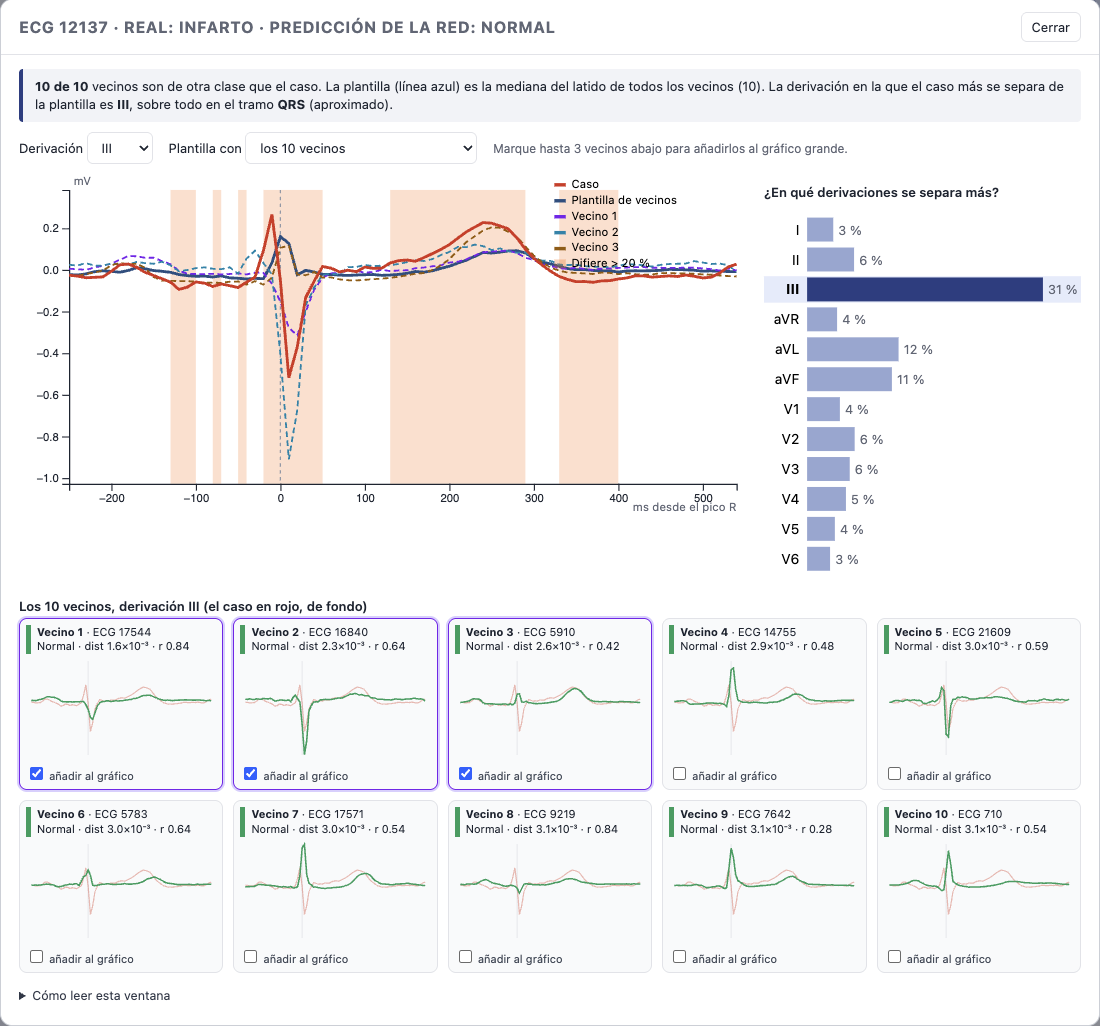
\includegraphics[width=0.62\textwidth]{figuras/ventana_comparacion.png}
\caption{Ventana de comparación (vista H) para el ECG 12137, infarto que la red clasifica como normal. En rojo, el latido medio del caso en la derivación III; en azul, la plantilla de sus 10 vecinos; las franjas marcan donde el caso difiere de la plantilla en más del 20\,\% de la amplitud del latido. A la derecha, la diferencia media por derivación; abajo, los 10 vecinos.}
\label{fig:comparacion}
\end{figure*}

\textbf{Caso C, la red y los vecinos no coinciden (ECG 12991).} La red duda entre STTC (48,1\,\%) y MI (46,6\,\%) y se inclina por STTC; en cambio, seis de sus diez vecinos son infartos y el kNN lo clasifica como MI con las tres distancias. Es uno de los 3 infartos, de los 83 que la red no detecta, que el kNN rescata. En V2, el caso y su vecino más cercano comparten una deflexión negativa profunda por latido. Aquí las probabilidades y los vecinos juntos dan más información que cada uno por separado: la probabilidad casi empatada y el vecindario mixto señalan un caso para revisar.

\textbf{Lo que muestran los tres casos.} Primero, el parecido en el espacio de 64 números no equivale a que las señales coincidan latido a latido en una derivación: el resumen se calcula con las 12 derivaciones y todo el registro, mientras que la figura compara una sola. Por eso la superposición sirve para revisar un caso, pero no prueba por sí sola que dos registros sean iguales. Segundo, la distancia al vecino distingue entre un acierto claro (caso A) y los demás, pero no separa un error en el que todos coinciden (caso B) de un caso dudoso (caso C): para eso sirven las probabilidades de la red y el voto de los vecinos.

\subsection{Patrones encontrados}
Al responder las preguntas del análisis, encontramos los siguientes patrones. Todos son descripciones de lo observado en este conjunto de datos y una sola ejecución del entrenamiento, no explicaciones causales.
\begin{enumerate}
\item \textbf{¿Los infartos se agrupan?} En parte. Con el resumen aprendido, dos coordenadas recuperan cerca del 57\,\% de los infartos, frente a 5\,\% con la señal cruda; forman una región reconocible, pero no aislada.
\item \textbf{¿Dónde falla la red?} Detecta 173 de 256 infartos; los errores van sobre todo a NORM (45) y STTC (31), y son mayores en infartos anteriores, en mujeres y con etapa desconocida.
\item \textbf{¿Por qué se pierden estos infartos?} Sus vecinos son en su mayoría de otra clase (13\,\% de acuerdo, frente a 76\,\% en los detectados) y están más lejos (cerca de 30\,\%). La distancia usada no lo explica: euclidiana y coseno dan los mismos vecinos y las otras dos distancias cambian pocos casos.
\item \textbf{¿Lo ven otros métodos?} K-means ubica 79 de los 83 infartos perdidos en grupos dominados por otra clase; DBSCAN no fue informativo.
\item \textbf{¿Tienen una huella en la señal?} Más débil, no distinta. Frente al latido normal típico, los infartos perdidos se desvían menos que los detectados, sobre todo en el QRS de III, aVF y aVL; y dentro de cada zona, menos en las derivaciones donde se espera la huella (inferiores II, III y aVF; anteriores V1 a V4). En prueba, los inferiores se detectan más (75\,\%) que los anteriores (55\,\%).
\item \textbf{¿Basta la distancia para revisar un caso?} No. En el estudio de casos, la distancia separa un acierto claro de los demás, pero para distinguir un error en que todos coinciden de un caso dudoso hacen falta las probabilidades de la red y el voto de los vecinos.
\end{enumerate}

% =====================================================================
\section{Discusión}

\subsection{¿Mejora el mapa aprendido al de la señal cruda?}
Sí, y por bastante. El Cuadro~\ref{tab:proyecciones} y la Fig.~\ref{fig:proyecciones} comparan cinco mapas de los registros de prueba. Con la señal cruda, los infartos quedan mezclados con todo lo demás: usando solo las dos coordenadas, un clasificador sencillo recupera apenas 5\,\% de los infartos y su AUC es de 0,54, casi azar. Con las 124 características calculadas a mano mejora (19\,\% de los infartos, AUC de 0,70), pero sigue siendo una nube sin estructura clara. Con el resumen que aprende la red, el mismo clasificador recupera entre 56 y 58\,\% de los infartos (AUC de 0,89--0,90) y la exactitud global sube de 0,53 a 0,77--0,79. Los infartos pasan a concentrarse en una región reconocible del mapa, aunque no aislada: en los bordes se mezclan con los ECG normales y con los de cambios ST-T.

Hay que leer esto con cuidado. El resumen de la red se entrena con las etiquetas y los mapas de la señal cruda y de las características no, así que la comparación mide el valor de aprender la representación y no una pelea entre iguales. Además, los valores de silhouette son bajos en todos los mapas (menos de 0,08): los infartos no forman un grupo aislado, sino una zona con vecinos de otras clases. UMAP y t-SNE dan resultados parecidos; t-SNE conserva algo mejor los vecindarios (trustworthiness de 0,986 frente a 0,969), pero no permite ubicar registros nuevos.

\subsection{¿Aporta algo la pérdida contrastiva?}
Poco, según nuestras medidas. En clasificación, la red con solo entropía cruzada es igual o mejor (AUC macro de 0,927 frente a 0,924; exactitud balanceada de 0,711 frente a 0,660; recall de HYP de 0,68 frente a 0,39). En el espacio de 64 números, la pérdida contrastiva sí ordena mejor los grupos (silhouette de 0,263 frente a 0,196), pero esa ventaja casi desaparece en el mapa 2D (kNN de 0,772 frente a 0,785; AUC de infarto de 0,896 frente a 0,890). Además, como solo hicimos una ejecución, no sabemos cuánto cambian estas cifras al repetir el entrenamiento, así que no afirmamos diferencias pequeñas. Usamos el modelo contrastivo en la plataforma por la mejor organización del espacio de 64 números; la conclusión honesta es que la mayor parte del beneficio viene de usar un resumen aprendido y no de la pérdida contrastiva en sí.

\subsection{¿Dónde falla el modelo con los infartos?}
En los registros de prueba, el modelo reconoce 173 de 256 infartos (recall de 0,68). Los errores van sobre todo a la clase normal (45 casos) y a STTC (31 casos). Los casos frontera más claros son errores seguros: en los 15 más confiables, el modelo asigna al infarto entre 2 y 13\,\% de probabilidad y a lo sumo 2 de sus 10 vecinos más parecidos son infartos. Que el modelo y sus vecinos coincidan puede significar que el infarto es sutil en el ECG o que la etiqueta es discutible; con estos datos no podemos distinguirlo.

Los errores no se reparten al azar (Cuadro~\ref{tab:errores}): se detectan peor los infartos anteriores (0,56 frente a 0,72 en los inferiores), los de mujeres (0,58 frente a 0,71 en hombres) y los de etapa desconocida (0,59 frente a 0,74 en etapa conocida). Una posible explicación de lo primero es que los infartos anteriores dejan cambios del segmento ST y la onda T que se parecen a los de la clase STTC, con la que se confunden; para el sexo y la etapa no tenemos una explicación respaldada por los datos y las dejamos como hipótesis para trabajo futuro.

\subsection{Limitaciones}
\begin{itemize}
\item Trabajamos con un solo diagnóstico por registro. Esto descarta el 24\,\% de los registros diagnosticados y el 80\,\% de los de hipertrofia, así que los resultados no representan los casos con varios diagnósticos a la vez.
\item Reportamos una sola ejecución del entrenamiento (una semilla). No medimos cuánto varían las métricas entre ejecuciones, por lo que las diferencias pequeñas entre modelos no son concluyentes.
\item El conjunto de prueba tiene solo 56 registros de hipertrofia; las cifras de esa clase son muy inciertas.
\item Las etiquetas de PTB-XL provienen de interpretaciones de ECG y no de una confirmación clínica independiente del infarto.
\item Los datos faltantes (por ejemplo, la etapa del infarto) se dejaron como categoría propia y no se imputaron; no podemos saber si faltan al azar, así que las comparaciones por etapa deben leerse con cautela.
\item No hicimos una evaluación con cardiólogos ni un estudio de usabilidad; la plataforma es un prototipo de análisis, no una herramienta de diagnóstico.
\item Probamos solo tres valores de $\varepsilon$ en DBSCAN, un solo $k$ en K-means y no reentrenamos con otro preprocesamiento de la señal (solo cambiamos la entrada de la red ya entrenada); por eso no descartamos que otro ajuste cambie la lectura de los grupos.
\item No usamos algoritmos de explicabilidad: no calculamos qué derivación o qué instante pesa más para el modelo. Las comparaciones por derivación (la ventana de comparación y el mapa de los infartos perdidos) describen la señal, no lo que usó la red. Además, con 256 infartos de prueba y un solo entrenamiento, el hallazgo sobre la huella en la señal es exploratorio.
\end{itemize}

% =====================================================================
\section{Conclusiones}
Construimos una plataforma de interpretabilidad visual para un modelo que detecta infartos en electrocardiogramas: dónde se ubican los infartos, qué vecinos y qué señal tiene cada caso y dónde falla el modelo. No usamos algoritmos de explicabilidad. Reúne siete vistas conectadas en tres niveles y tres ventanas emergentes, y responde a tres tareas: explorar cohortes, comprobar si los infartos se agrupan y revisar los casos frontera.

Cinco resultados resumen el trabajo. Primero, un resumen numérico aprendido por la red produce un mapa mucho más informativo que la señal cruda o las características calculadas a mano: con solo dos coordenadas se recupera cerca del 57\,\% de los infartos, frente a 5\,\% con la señal cruda. Segundo, la pérdida contrastiva no mejora de forma clara ni la clasificación ni el mapa 2D; el beneficio viene de usar un resumen aprendido. Tercero, el modelo detecta cerca de dos de cada tres infartos y falla más con los infartos anteriores, en mujeres y con etapa desconocida, errores que un número global de acierto no deja ver. Cuarto, los infartos mal clasificados tienen vecinos de otra clase y algo más lejanos, y ni cambiar la distancia ni agrupar con K-means o DBSCAN los separa: el error está en la representación que aprendió la red. Quinto, en la señal, los infartos perdidos conservan la forma general de un infarto, pero se desvían menos del latido normal típico que los detectados, sobre todo en el QRS de las derivaciones III, aVF y aVL; es una descripción del error y no una explicación de su causa.

Como trabajo futuro, proponemos incluir los registros con varios diagnósticos, repetir el entrenamiento con varias semillas, aplicar algoritmos de explicabilidad para saber qué derivaciones y qué instantes usa la red, validar los casos con cardiólogos, y usar validación cruzada para estudiar si algunas etiquetas dudosas explican parte de los errores. El funcionamiento de la plataforma se muestra en el video que acompaña este informe.

% =====================================================================
\begin{thebibliography}{99}
\bibitem{alvarenga} J. Alvarenga, M. Batista, S. F. Adorno y L. Gustavo, «CrimAnalyzer: Understanding crime patterns in São Paulo city,» arXiv:2010.06517, 2020.
\bibitem{cao} N. Cao, C. Lin, Q. Zhu, Y.-R. Lin, X. Teng y X. Wen, «Voila: Visual anomaly detection and monitoring with streaming spatiotemporal data,» \emph{IEEE Trans. Vis. Comput. Graph.}, vol. 24, n.º 1, pp. 23--33, 2017.
\bibitem{hannun} A. Y. Hannun \emph{et~al.}, «Cardiologist-level arrhythmia detection and classification in ambulatory electrocardiograms using a deep neural network,» \emph{Nature Medicine}, vol. 25, n.º 1, pp. 65--69, 2019. doi:10.1038/s41591-018-0268-3.
\bibitem{khosla} P. Khosla \emph{et~al.}, «Supervised contrastive learning,» en \emph{Advances in Neural Information Processing Systems}, vol. 33, pp. 18661--18673, 2020.
\bibitem{kiyasseh} D. Kiyasseh, T. Zhu y D. A. Clifton, «CLOCS: Contrastive learning of cardiac signals across space, time, and patients,» en \emph{Proc. Int. Conf. Machine Learning (ICML)}, PMLR vol. 139, pp. 5606--5615, 2021.
\bibitem{luo} X. Luo, R. Jiang, B. Yang, H. Qin y H. Hu, «Air quality visualization analysis based on multivariate time series data feature extraction,» \emph{Journal of Visualization}, vol. 27, n.º 4, pp. 567--584, 2024.
\bibitem{mcinnes} L. McInnes, J. Healy y J. Melville, «UMAP: Uniform manifold approximation and projection for dimension reduction,» arXiv:1802.03426, 2018.
\bibitem{velumani} R. Palaniyappan Velumani, M. Xia, J. Han, C. Wang, A. K. H. Lau y H. Qu, «AQX: Explaining air quality forecast for verifying domain knowledge using feature importance visualization,» en \emph{Proc. Int. Conf. Intelligent User Interfaces (IUI)}, pp. 720--733, 2022.
\bibitem{qu} D. Qu, C. Lv, Y. Lin, H. Zhang y R. Wang, «AirLens: Multi-level visual exploration of air quality evolution in urban agglomerations,» \emph{Computer Graphics Forum}, vol. 41, n.º 3, pp. 223--234, 2022.
\bibitem{strodthoff} N. Strodthoff, P. Wagner, T. Schaeffter y W. Samek, «Deep learning for ECG analysis: Benchmarks and insights from PTB-XL,» \emph{IEEE J. Biomed. Health Inform.}, vol. 25, n.º 5, pp. 1519--1528, 2021. doi:10.1109/JBHI.2020.3022989.
\bibitem{vandermaaten} L. van der Maaten y G. Hinton, «Visualizing data using t-SNE,» \emph{J. Mach. Learn. Res.}, vol. 9, pp. 2579--2605, 2008.
\bibitem{wagner} P. Wagner \emph{et~al.}, «PTB-XL, a large publicly available electrocardiography dataset,» \emph{Scientific Data}, vol. 7, art. 154, 2020. doi:10.1038/s41597-020-0495-6.
\end{thebibliography}

\end{document}
